\documentclass[review]{elsarticle}

\usepackage{parskip}
\usepackage[running]{lineno}
\usepackage{mathptmx}     
\usepackage{latexsym}
\usepackage{hyperref}
\usepackage{setspace}
%\usepackage[section]{placeins}
\doublespacing
\usepackage{bm,amsmath,bbm,amsfonts,nicefrac,latexsym,amsmath,amsfonts,amsbsy,amscd,amsxtra,amsgen,amsopn,bbm,amsthm,amssymb,graphicx, color, caption, subcaption, pbox, fixltx2e}
\usepackage{epstopdf}
\usepackage[margin=0.8in]{geometry}
%\modulolinenumbers[2]


\journal{Agriculture and Forest Meteorology}

%%%%%%%%%%%%%%%%%%%%%%%
%% Elsevier bibliography styles
%%%%%%%%%%%%%%%%%%%%%%%
%% To change the style, put a % in front of the second line of the current style and
%% remove the % from the second line of the style you would like to use.
%%%%%%%%%%%%%%%%%%%%%%%

%% Numbered
%\bibliographystyle{model1-num-names}

%% Numbered without titles
%\bibliographystyle{model1a-num-names}

%% Harvard
\bibliographystyle{model2-names.bst}\biboptions{authoryear}

%% Vancouver numbered
%\usepackage{numcompress}\bibliographystyle{model3-num-names}

%% Vancouver name/year
%\usepackage{numcompress}\bibliographystyle{model4-names}\biboptions{authoryear}

%% APA style
%\bibliographystyle{model5-names}\biboptions{authoryear}

%% AMA style
%\usepackage{numcompress}\bibliographystyle{model6-num-names}

%% `Elsevier LaTeX' style
%\bibliographystyle{elsarticle-num}
%%%%%%%%%%%%%%%%%%%%%%%

\begin{document}

\begin{frontmatter}

\title{Investigating the role of {\color{red}prior *rev3} and observation error correlations in improving a model forecast of forest carbon balance using four dimensional variational data assimilation.}
%\tnotetext[mytitlenote]{Fully documented templates are available in the elsarticle package on \href{http://www.ctan.org/tex-archive/macros/latex/contrib/elsarticle}{CTAN}.}

%% Group authors per affiliation:
%\author{Elsevier\fnref{myfootnote}}
%\address{Radarweg 29, Amsterdam}
%\fntext[myfootnote]{Since 1880.}

%% or include affiliations in footnotes:
\author[address1]{Ewan M. Pinnington\corref{mycorrespondingauthor}}
\cortext[mycorrespondingauthor]{Corresponding author}
\ead{e.m.pinnington@pgr.reading.ac.uk}

\author[address3]{Eric Casella}

\author[address1,address2]{Sarah L. Dance}

\author[address1,address2,address4]{Amos S. Lawless}

\author[address3]{James I. L. Morison}

\author[address1,address2,address4]{Nancy K. Nichols}

\author[address3]{Matthew Wilkinson}

\author[address1,address4]{Tristan L. Quaife}


\address[address1]{Department of Meteorology, University of Reading, Reading, UK}
\address[address2]{Department of Mathematics and Statistics, University of Reading, Reading, UK}
\address[address3]{Centre for Sustainable Forestry and Climate Change, Forest Research, Alice Holt, Farnham, UK}
\address[address4]{National Centre for Earth Observation, University of Reading, Reading, UK}


\begin{abstract}
Efforts to implement variational data assimilation routines with functional ecology models and land surface models have been limited, with sequential and Markov chain Monte Carlo data assimilation methods being prevalent. When data assimilation has been used with models of carbon balance, background ``prior" errors {\color{red}(in the initial state and parameter values) *rev3} and observation errors have largely been treated as independent and uncorrelated. Correlations between background errors have long been known to be a key aspect of data assimilation in numerical weather prediction. More recently, it has been shown that accounting for correlated observation errors in the assimilation algorithm can considerably improve data assimilation results and forecasts. In this paper we implement a Four-Dimensional Variational data assimilation (4D-Var) scheme with a simple model of forest carbon balance, for joint parameter and state estimation and assimilate daily observations of Net Ecosystem $\text{CO}_{2}$ Exchange (NEE) taken at the Alice Holt forest $\text{CO}_2$ flux site in Hampshire, UK. We then investigate the effect of specifying correlations between parameter and state variables in background error statistics and the effect of specifying correlations in time between observation error statistics. The idea of including these correlations in time is new and has not been previously explored in carbon balance model data assimilation. In data assimilation, background and observation error statistics are often described by the background error covariance matrix and the observation error covariance matrix. We outline novel methods for creating correlated versions of these matrices, using a set of previously postulated dynamical constraints to include correlations in the background error statistics and a Gaussian correlation function to include time correlations in the observation error statistics. The methods used in this paper will allow the inclusion of time correlations between many different observation types in the assimilation algorithm, meaning that previously neglected information can be accounted for. {\color{red}In our experiments we assimilate a single year of NEE observations and then run a forecast for the next 14 years. *rev3} We compared the results using our new correlated background and observation error covariance matrices and those using diagonal covariance matrices. We found that using the new correlated matrices reduced the root mean square error in the $14$ year forecast of daily NEE by $44\%$ decreasing from $4.22~\text{gCm}^{-2}\text{day}^{-1}$ to $2.38~\text{gCm}^{-2}\text{day}^{-1}$.     
\end{abstract}

\begin{keyword}
Carbon cycle \sep DALEC \sep Eddy covariance \sep Error covariance \sep Parameter estimation
%\MSC[2010] 00-01\sep  99-00
\end{keyword}

\end{frontmatter}

\linenumbers

\section{Introduction} \label{sec:intro}

%\subsection{Tree blurb}
The land surface and oceans are responsible for removing around half of all human emitted carbon-dioxide from the atmosphere and therefore mediate the effect of anthropogenic induced climate change. Terrestrial ecosystem carbon uptake is the least understood process in the global carbon cycle \citep{ciais2014carbon}. It is therefore vital that we improve understanding of the carbon uptake of terrestrial ecosystems and their response to climate change in order to better constrain predictions of future carbon budgets. Observations of the Net Ecosystem Exchange (NEE) of CO$_{2}$ between terrestrial ecosystems and the atmosphere are now routinely made at flux tower sites world-wide, at sub-hourly resolution and covering multiple years \citep{baldocchi2008turner}, providing a valuable resource for carbon balance model validation and data assimilation.

%\subsection{DA paragraph}
Data assimilation is the process of combining a mathematical model with observations in order to improve the estimate of the state of a system. Data assimilation has successfully been used in many applications to significantly improve model state and forecasts. Perhaps the most important application has been in numerical weather prediction where data assimilation has contributed to the forecast accuracy being increased at longer lead times, with the four day forecast in 2014 having the same level of accuracy as the one day forecast in 1979 \citep{bauer2015quiet}. This increase in forecast skill is obviously not solely due to data assimilation but also increased quality and resolution of observations along with improvements in model structure, however the introduction and evolution of data assimilation has played a large part \citep{dee2011era}. The current method implemented at many leading operational numerical weather prediction centres is known as Four-Dimensional Variational data assimilation (4D-Var) \citep{QJ:QJ2652, QJ:QJ2054}, which has been shown to be a significant improvement over its predecessor three-dimensional variational data assimilation \citep{lorenc2005does}. Variational assimilation techniques minimise a cost function to find the optimal state of a system given all available knowledge of errors in the model and observations. The minimisation routine typically requires the derivative of the model which can sometimes prove difficult to calculate. Using techniques such as automatic-differentiation \citep{renaud1997automatic} can reduce the time taken to implement the derivative of a model. 

In numerical weather prediction data assimilation has been predominately used for state estimation whilst keeping parameters fixed. {\color{red}This is because numerical weather prediction is mainly dependent on the initial state with model physics being well understood. Ecosystem carbon cycle models are more dependent on finding the correct set of parameters to describe the ecosystem of interest \citep{luo2015predictability}. This is possibly why Monte Carlo Markov chain (MCMC) data assimilation methods have been used more with ecosystem carbon cycle models. *rev2} Variational data assimilation can be used for joint parameter and state estimation by augmenting the state vector with the parameters \citep{navon1998practical}. By including the parameters in the state vector we must also specify error statistics and error correlations for them. \citet{smith2009variational} show that the prescription of these error statistics and their correlations can have a significant impact on parameter-state estimates obtained from the assimilation.

%\subsection{DALEC and ecosystem models with data assimilation (draw out gaps):}
Many different observations relevant to the carbon balance of forests have now been combined with functional ecology models, using data assimilation, in order to improve our knowledge of ecological systems \citep{zobitz2011primer, fox2009reflex, richardson2010estimating, Quaife2008, Zobitz2014, Niu2014}. Two such models that have been used extensively with data assimilation are the Data Assimilation Linked Ecosystem Carbon (DALEC) model \citep{williams2005improved} and the Simplified Photosynthesis and Evapo-Transpiration (SIPNET) model \citep{braswell2005estimating}. Nearly all data assimilation routines built with these models have used sequential and Monte Carlo Markov chain (MCMC) data assimilation methods with the exception of a variational routine being implemented for DALEC by \citet{delahaies2013regularization}. There have been examples of global land surface models being implemented with variational methods such as the ORganizing Carbon and Hydrology In Dynamic EcosystEms model (ORCHIDEE) \citep{Krinner2005} and the Biosphere Energy Transfer HYdrology scheme (BETHY) in a Carbon Cycle Data Assimilation System (CCDAS) \citep{Kaminski2013}. These examples have mainly been used to assimilate data from satellite and atmospheric $\text{CO}_{2}$ observations with only a few cases where site level data has also been assimilated \citep{Verbeeck2011, Bacour2015}.

Background errors (describing our knowledge of error in prior model estimates before data assimilation) and observation errors have largely been treated as uncorrelated and independent in ecosystem model data assimilation schemes. In 3D and 4DVar schemes background and observation errors are represented by the error covariance matrices \textbf{B} and \textbf{R} respectively. The off-diagonal elements of these matrices indicate the correlations between errors in the parameter and state variables for \textbf{B} and the correlations between observation errors for \textbf{R}. In the assimilation, the off-diagonal terms in the \textbf{B} matrix act to spread information between the state and augmented parameter variables \citep{kalnay2003atmospheric}. This means that assimilating observations of one state variable can act to update different state and parameter variables in the assimilation when correlations are included in \textbf{B}. In 4D-Var the \textbf{B} matrix is propagated implicitly by the forecast model, so that even a propagated diagonal \textbf{B} matrix can develop correlations throughout an assimilation window. These correlations will only be in the propagated \textbf{B} matrix, with the \textbf{B} matrix valid at the initial time remaining unchanged. Including correlations in \textbf{B} has been shown to significantly improve data assimilation results in numerical weather prediction \citep{bannister2008review}. 

Including correlations between observation errors has only started to be explored recently in numerical weather prediction, with \textbf{R} still often treated as diagonal \citep{Stewart2013}. Including some correlation structure in \textbf{R} has been shown to improve forecast accuracy \citep{weston2014accounting}. Currently the correlations included in \textbf{R} have been mainly between observations made at the the same time rather than correlations between observations throughout time. When assimilating observations, data streams with many more observations can have a greater impact on the assimilation than those with fewer observations. In \citet{richardson2010estimating} this problem is discussed when assimilating large numbers of NEE observations along with smaller numbers of leaf area index and soil respiration observations. To address this problem Richardson et al. uses a cost function that calculates the product of the departures from the observations rather than a cost function which sums these departures, giving a relative rather than absolute measure of the goodness-of-fit to the observations. This problem is also encountered in \citet{Bacour2015} when assimilating daily eddy covariance data with weekly observations of the FrAction of Photosynthetically Active Radiation (FAPAR). In \citet{Bacour2015} the error in observations of FAPAR is divided by two in order to give these less frequent observations more weight in the assimilation algorithm. Specifying serial time correlations between observations represents another way of addressing this problem, whilst also adding valuable information to the data assimilation routine. Including serial correlations between observations of the same quantity decreases the impact of these observations \citep{jarvinen1999variational} therefore increasing the impact of less frequent observations. 

%\subsection{What does this paper do/results:}
In this paper we implement the new version of DALEC (DALEC2 \citep{Bloom2015}) in a 4D-Var data assimilation scheme for joint state and parameter estimation, assimilating daily NEE observations from the Alice Holt flux site in Hampshire, UK \citep{wilkinson2012inter}. This assimilation scheme is then subjected to rigorous testing to ensure correctness. A new method is outlined for including parameter and state correlations in the background ``prior" error covariance matrix. Currently parameter and state error statistics are largely treated as independent and uncorrelated when data assimilation has been used with models of carbon balance. We also introduce a novel method for including serial time correlations in the observation error covariance matrix. The idea of including time correlations between observation error statistics is new and has not been previously explored in carbon balance model data assimilation. These correlated matrices are then used in a series of experiments in order to examine the effect that including correlations in the assimilation scheme has on the results. We show that specifying parameter and state correlations in the prior knowledge and serial correlations between observation errors can significantly improve the fit of the predicted carbon balance to observations with the root mean square error in the 14 year forecast of daily NEE decreasing by $44\%$ from $4.22~\text{gCm}^{-2}\text{day}^{-1}$ to $2.38~\text{gCm}^{-2}\text{day}^{-1}$.

\section{Model and Data Assimilation Methods}

\subsection{Alice Holt research forest}

Alice Holt Forest is a research forest area managed by the UK Forestry Commission located in Hampshire, SE England. Forest Research has been operating a $\text{CO}_{2}$ flux measurement tower in a portion of the forest, the Straits Inclosure, since 1998 so it is one of the longer forest site $\text{CO}_2$ flux records, globally. The Straits Inclosure is a $90 \text{ha}$ area of managed deciduous broadleaved plantation woodland, presently approximately $80$ years old, on a surface water gley soil. The majority of the canopy trees are oak (\textit{Quercus robur} L.), with an understory of hazel (\textit{Corylus avellana} L.) and hawthorn (\textit{Crataegus monogyna} Jacq.); but there is a small area of conifers (\textit{Pinus nigra} J. F. Arnold) within the tower measurement footprint area in some weather conditions. Further details of the Straits Inclosure site and the measurement procedures are given in \citet{wilkinson2012inter}, together with analysis of stand-scale $30$ minute average net $\text{CO}_{2}$ fluxes (NEE) measured by standard eddy covariance methods from 1998-2011. The data used here span from January 1999 to December 2013, and consist of the NEE fluxes and meteorological driving data of temperatures, irradiance and atmospheric $\text{CO}_2$ concentration. The original NEE data were subjected to normal quality control procedures, including $u^{*}$ filtering to remove unreliable data when there were low turbulence night time conditions, as described in \citet{wilkinson2012inter}, but were not gap-filled. To compute daily NEE observations we take the sum over the 48 measurements made each day. We only select days where there is no missing data and over $90\% $ of $\text{CO}_2$ flux observations have a quality control flag associated with the best observations and no observations associated with the worst from the EddyPro flux processing software \citep{eddypro}.

\subsection{The DALEC2 model}

The DALEC2 model is a simple process-based model describing the carbon balance of a forest ecosystem \citep{Bloom2015} and is the new version of the original DALEC \citep{williams2005improved}. The model is constructed of six carbon pools (labile ($C_{lab}$), foliage ($C_f$), fine roots ($C_r$), woody stems and coarse roots ($C_w$), fresh leaf and fine root litter ($C_l$) and soil organic matter and coarse woody debris ($C_s$)) linked via fluxes. The aggregated canopy model (ACM) \citep{williams1997predicting} is used to calculate daily gross primary production ($GPP$) of the forest, taking meteorological driving data and the modelled leaf area index (a function of $C_f$) as arguments. Figure~\ref{fig:DALEC_mod} shows a schematic of how the carbon pools are linked in DALEC2.   

\begin{figure}[ht]
    \centering
    \includegraphics[width=0.5\textwidth]{dalec2diag.pdf}
    \caption{Representation of the fluxes in the DALEC2 carbon balance model. Green arrows represent C allocation, purple arrows represent litter fall and decomposition fluxes, blue arrows represent respiration fluxes and the red arrow represents the influence of leaf area index in the $GPP$ function.} \label{fig:DALEC_mod}
\end{figure}

The model equations for the carbon pools at day $i$ are as follows:

\begin{align}
GPP^{i} &= ACM(C_{fol}^{i-1}, c_{lma}, c_{eff}, \Psi) \label{GPP}
\\C_{lab}^{i}&=C_{lab}^{i-1}+(1-f_{auto})(1-f_{fol})f_{lab}GPP^{i}-\Phi _{on}C_{lab}^{i-1}, \label{daleclab}
\\C_{fol}^{i}&=C_{fol}^{i-1}+\Phi_{on}C_{lab}^{i-1}+(1-f_{auto})f_{fol}GPP^{i}-\Phi_{off}C_{fol}^{i-1}, \label{dalec1}
\\C_{roo}^{i}&=C_{roo}^{i-1}+(1-f_{auto})(1-f_{fol})(1-f_{lab})f_{roo}GPP^{i}-\theta_{roo}C_{roo}^{i-1}, 
\\C_{woo}^{i}&=C_{woo}^{i-1}+(1-f_{auto})(1-f_{fol})(1-f_{lab})(1-f_{roo})GPP^{i}-\theta_{woo}C_{woo}^{i-1}, 
\\C_{lit}^{i}&=C_{lit}^{i-1}+\theta_{roo}C_{roo}^{i-1}+\Phi_{off}C_{fol}^{i-1}-(\theta_{lit}+\theta_{min})e^{\Theta T^{i-1}}C_{lit}^{i-1}, 
\\C_{som}^{i}&=C_{som}^{i-1}+\theta_{woo}C_{woo}^{i-1}+\theta_{min}e^{\Theta T^{i-1}}C_{lit}^{i-1}-\theta_{som}e^{\Theta T^{i-1}}C_{som}^{i-1}, \label{dalec5}
\end{align}
where $T^{i-1}$ is the daily mean temperature, $\Psi$ represents the meteorological driving data used in the $GPP$ function and $\Phi_{on} / \Phi_{off}$ are functions controlling leaf-on and leaf-off. {\color{red} Descriptions for each model parameter used in equations \eqref{GPP} to \eqref{dalec5} are included in the appendix in table~\ref{table:xbvars}. *rev3} DALEC2 differs from the original DALEC in that it can be parameterised for both deciduous and evergreen sites with $\Phi_{on}$ and $\Phi_{off}$ being able to reproduce the phenology of either type of site. The full details of this version of DALEC can be found in \cite{Bloom2015}. 

\subsection{4D-Var} \label{4dvar}

Following the approach of \citet{Smith2011436} for three-dimensional variational data assimilation, we consider the discrete nonlinear dynamical system given by
\begin{linenomath}
\begin{equation}
\textbf{z}_{i} = \textbf{f}_{i-1\rightarrow i}(\textbf{z}_{i-1}, \textbf{p}_{i-1}),
\end{equation}
\end{linenomath}
where \( \textbf{z}_{i} \in \mathbb{R}^{n} \) is the state vector at time \( t_i \), \(\textbf{f}_{i-1 \rightarrow i}\) is the nonlinear model operator propagating the state at time \(t_{i-1}\) to time \(t_{i}\) for \(i = 1, 2, \dots, N\) and \(\textbf{p}_{i-1} \in \mathbb{R}^{q}\) is a vector of \(q\) model parameters at time \(t_{i-1}\). For DALEC2 the state vector \(\textbf{z}_{i}=(C_{lab}^{i}, C_{for}^{i}, C_{roo}^{i}, C_{woo}^{i}, C_{lit}^{i}, C_{som}^{i})^{T}\), with the parameters shown in table~\ref{table:xbvars}. The model parameters are not updated by the nonlinear model operator, therefore the evolution of the parameters is given by,
\begin{linenomath}
\begin{equation}
\textbf{p}_{i} = \textbf{p}_{i-1}, 
\end{equation}
\end{linenomath}
for $i= 1, 2, \dots, N$. We define the new vector $\textbf{x}$ by joining the parameter vector $\textbf{p}$ with the model state vector $\textbf{z}$, giving us the augmented state vector
\begin{linenomath}
\begin{equation}
\textbf{x} =
\begin{pmatrix}
\textbf{p} \\
\textbf{z}
\end{pmatrix}
\in \mathbb{R}^{q+n}.
\end{equation}
\end{linenomath}
We define the augmented system model by
\begin{linenomath}
\begin{equation}
\textbf{x}_{i} = \textbf{m}_{i-1 \rightarrow i}(\textbf{x}_{i-1}), \label{eqn:nonlinmod}
\end{equation}
\end{linenomath}
where
\begin{linenomath}
\begin{equation}
\textbf{m}_{i-1\rightarrow i}(\textbf{x}_{i-1}) =
\begin{pmatrix}
\textbf{p}_{i-1} \\
\textbf{f}_{i-1\rightarrow i}(\textbf{z}_{i-1}, \textbf{p}_{i-1})
\end{pmatrix}
=
\begin{pmatrix}
\textbf{p}_{i} \\
\textbf{z}_{i}
\end{pmatrix}
\in \mathbb{R}^{q+n}.
\end{equation}
\end{linenomath}
The available observations at time $t_{i}$ are represented by the vector $\textbf{y}_{i} \in \mathbb{R}^{r_{i}}$ which are related to the augmented state vector through the equation
\begin{linenomath}
\begin{equation}
\textbf{y}_{i}=\textbf{h}_{i}(\textbf{x}_{i})+ \mathbf{ \epsilon}_{i},
\end{equation} 
\end{linenomath}
where $\textbf{h}_{i}: \mathbb{R}^{q+n} \rightarrow \mathbb{R}^{r_{i}}$ is the observation operator mapping the augmented state vector to observation space and $\mathbf{\epsilon}_{i} \in \mathbb{R}^{r_{i}}$ represents the observation errors. These errors are usually assumed to be unbiased, Gaussian and serially uncorrelated with known covariance matrices $\textbf{R}_{i}$.

We assume that at time $t_{0}$ we have an initial estimate to the augmented state, usually referred to as the background vector denoted $\textbf{x}^{b}$. This background is assumed to have unbiased, Gaussian errors with known covariance matrix $\textbf{B}$. {\color{red} This matrix is not altered during the assimilation process. *rev3} In 4D-Var we aim to find the initial state that minimises the weighted least squares distance to the background while minimising the weighted least squares distance of the model trajectory to the observations over the time window $t_{0}, \dots, t_{N}$ \citep{lawless2013}. We do this by finding the state $\textbf{x}^{a}_{0}$ at time $t_{0}$ that minimises the cost function
\begin{linenomath}
\begin{equation}
J(\textbf{x}_0) = \frac{1}{2}(\textbf{x}_0-\textbf{x}^b)^{T}\textbf{B}^{-1}(\textbf{x}_0-\textbf{x}^b)+\frac{1}{2}\sum_{i=0}^{N}(\textbf{y}_i-\textbf{h}_i(\textbf{x}_i))^{T}\textbf{R}_{i}^{-1}(\textbf{y}_i-\textbf{h}_i(\textbf{x}_i)),
\end{equation}
\end{linenomath}
subject to the augmented states $\textbf{x}_{i}$ satisfying the nonlinear dynamical model \eqref{eqn:nonlinmod}. The state that minimises the cost function, $\textbf{x}^{a}_{0}$, is commonly called the analysis. This state is found using a minimisation routine that takes as its input arguments the cost function, the background vector ($\textbf{x}^{b}$) and also the gradient of the cost function given as,
\begin{linenomath}
\begin{equation}
\nabla J(\textbf{x}_0) = \textbf{B}^{-1}(\textbf{x}_0-\textbf{x}^{b})-\sum_{i=0}^{N}\textbf{M}_{i,0}^{T}\textbf{H}_i^{T}\textbf{R}_{i}^{-1}(\textbf{y}_i-\textbf{h}_i(\textbf{x}_i))
\end{equation}
\end{linenomath}
where $\textbf{H}_i = \frac{\partial \textbf{h}_i(\textbf{x}_i)}{\partial\textbf{x}_i}$ is the linearized observation operator and $\mathbf{M}_{i,0}=\mathbf{M}_{i-1}\mathbf{M}_{i-2}\cdots\mathbf{M}_0$ is the tangent linear model with $\mathbf{M}_i=\frac{\partial \textbf{m}_{i-1\rightarrow i}(\textbf{x}_{i})}{\partial \textbf{x}_{i}}$. In practice $\nabla J(\textbf{x}_0)$ is calculated using the method of Lagrange multipliers as shown in \citet{lawless2013}. We can rewrite the cost function and its gradient to avoid the sum notation as,
\begin{linenomath}
\begin{equation}
J(\textbf{x}_0) = \frac{1}{2}(\textbf{x}_0-\textbf{x}^b)^{T}\textbf{B}^{-1}(\textbf{x}_0-\textbf{x}^b)+\frac{1}{2}(\hat{\textbf{y}}-\hat{\textbf{h}}(\textbf{x}_0))^{T}\hat{\textbf{R}}^{-1}(\hat{\textbf{y}}-\hat{\textbf{h}}(\textbf{x}_0)) \label{costfn}
\end{equation}
\end{linenomath}
and
\begin{linenomath}
\begin{equation}
\nabla J(\textbf{x}_0) = \textbf{B}^{-1}(\textbf{x}_0-\textbf{x}^b)-\hat{\mathbf{H}}^{T}\hat{\textbf{R}}^{-1}(\hat{\textbf{y}}-\hat{\textbf{h}}(\textbf{x}_0)), \label{gradcostfn}
\end{equation}
\end{linenomath}
where,
\begin{linenomath}
\begin{equation}
\hat{\textbf{y}}=
\begin{pmatrix}
\textbf{y}_0 \\
\textbf{y}_1\\
\vdots \\
\textbf{y}_N
\end{pmatrix},
\hspace{1mm}
\hat{\textbf{h}}(\textbf{x}_0)=
\begin{pmatrix}
\textbf{h}_0(\textbf{x}_0) \\
\textbf{h}_1(\textbf{m}_{0\rightarrow 1}(\mathbf{x}_{0}))\\
\vdots \\
\textbf{h}_N(\textbf{m}_{0\rightarrow N}(\mathbf{x}_{0}))
\end{pmatrix},
\hspace{1mm}
\hat{\mathbf{R}}=
\begin{pmatrix}
\mathbf{R}_{0, 0} & \mathbf{R}_{0, 1} & \dots & \mathbf{R}_{0, N} \\
\mathbf{R}_{1, 0} & \mathbf{R}_{1, 1} & \dots & \mathbf{R}_{1, N} \\
\vdots & \vdots & \ddots & \vdots \\
\mathbf{R}_{N, 0} & \mathbf{R}_{N, 1} & \dots & \mathbf{R}_{N, N}
\end{pmatrix}
\hspace{1mm} \text{and} \hspace{3mm}
\hat{\mathbf{H}}=
\begin{pmatrix}
\mathbf{H}_0 \\
\mathbf{H}_1\mathbf{M}_0\\
\vdots \\
\mathbf{H}_N\mathbf{M}_{N,0}
\end{pmatrix}.
\end{equation}
\end{linenomath}

Solving the cost function in this form also allows us to build serial time correlations into the observation error covariance matrix $\hat{\mathbf{R}}$. The off-diagonal blocks of $\hat{\mathbf{R}}$ represent correlations in time between assimilated observations and are usually taken to be zero, in section~\ref{sec:corR} we show how these off-diagonal blocks can be specified. {\color{red} We can also calculate the posterior or analysis error covariance matrix after assimilation as, *rev3}
\begin{linenomath}
\begin{equation}
\mathbf{A} = (\textbf{B}^{-1} + \hat{\mathbf{H}}^{T}\hat{\textbf{R}}^{-1}\hat{\mathbf{H}})^{-1}, \label{eqn:Amat}
\end{equation}
\end{linenomath}
we can use this matrix to estimate the uncertainty in our initial parameter and state variables after assimilation.
%Forecast skill score, $SS = 1 - \frac{MSE_{forecast}}{MSE_{ref}}$, http://en.wikipedia.org/wiki/Forecast_skill

\subsection{Implementation and testing of 4D-Var system} \label{sec:implement4dvar}

In our DALEC2 4D-Var scheme we are performing joint parameter and state estimation. {\color{red} Typically MCMC techniques have been used for joint parameter and state estimation with functional ecology models, such as DALEC2. However 4D-Var has been used for joint parameter and state estimation with global carbon cycle models \citep{Kaminski2013}. We are optimising the state and parameter values of DALEC2 at the initial time. *rev1} The augmented state vector, $\textbf{x}_0$, corresponds to the vector of the 17 model parameters and 6 initial carbon pool values, which can be found in the appendix in table~\ref{table:xbvars}. Here the nonlinear model (DALEC2) only updates the initial carbon pool values when evolving the augmented state vector forward in time with the parameters being held constant. To find the background estimate, $\textbf{x}^{b}$, to the augmented state vector we can either use a previous DALEC2 model forecast estimate of the state of the system for the site (when available) or use expert elicitation to define likely state and parameter values and ranges for the site. The background vector $(\textbf{x}^b)$ and its corresponding standard deviations (see table~\ref{table:xbvars}) used in this paper were provided from existing runs of the the CARbon DAta-MOdel fraMework (CARDAMOM) \citep{Exbrayat2015}. This is a dataset derived from satellite observations of leaf area index which provides a reasonable first guess to DALEC2 state and parameter values for the Alice Holt research site. In this paper we assimilate observations of daily NEE. From \citet{Richardson200838} the measurement error in observations of daily NEE is between $0.2$ to $0.8~\text{gCm}^{-2}\text{day}^{-1}$.  \citet{Richardson200838} also shows that flux errors are heteroscedastic. We assume a constant standard deviation of $0.5~\text{gCm}^{-2}\text{day}^{-1}$ in the assimilated observations of daily NEE as we found this standard deviation gave the best weighting to the observations in the assimilation algorithm, producing the best results for the forecast of NEE after assimilation. Assuming this constant standard deviation also allows for correlations in time between observation errors to be included more easily. {\color{red} Ignoring the heteroscedastic nature of NEE errors may influence results by giving observations of larger magnitude a higher weight than would be realistic. Future work should try to incorporate the heteroscedastic nature of NEE errors. *rev3}

In order to find the tangent linear model (TLM) for DALEC2 it is necessary to find the derivative of the model at each time step with respect to the 17 model parameters and the 6 carbon pools. We use the AlgoPy automatic differentiation package \citep{Walter2013} in Python to calculate the TLM at each time step. This package uses forward mode automatic differentiation to calculate the derivative of the model. In the following tests we use a diagonal approximation to the background and observation error covariance matrices so that, 
$\textbf{B}_{diag}=\text{diag}(\bm{\sigma}_b)^2$ and $\hat{\textbf{R}}_{diag}=\text{diag}(\bm{\sigma}_o )^2$,
where $\bm{\sigma}_b$ is the vector of background standard deviations found in table~\ref{table:xbvars} and $\bm{\sigma}_o$ is the vector of observational standard deviations, for a single observation of NEE $\sigma_o=0.5~\text{gCm}^{-2}\text{day}^{-1}$. {\color{red}To minimise the cost function we use the truncated Newton method \citep{Nocedal1999} from the Python package Scipy.optimize \citep{scipy2015}. This method is able to converge on a unique solution when assimilating a single year of NEE observations. *rev3} In sections \ref{sec:testtlm} to \ref{sec:testgrad} we show tests of our scheme. 


\subsubsection{Test of tangent linear model} \label{sec:testtlm}

We can have confidence that our implementation of the TLM for DALEC2 is correct as it passes the following relevant tests \citep{Li1994}. In 4D-Var we assume the tangent linear hypothesis,
\begin{linenomath}
\begin{equation}
\textbf{m}_{0\rightarrow i}(\mathbf{x}_0+\gamma \delta\mathbf{x}_0) \approx \textbf{m}_{0 \rightarrow i}(\mathbf{x}_0) +\gamma \mathbf{M}_{i,0} \delta\mathbf{x}_0, \label{TLH}
\end{equation}
\end{linenomath}
where $\delta\mathbf{x}_0$ is a perturbation of the initial augmented state $\textbf{x}_{0}$ and $\gamma$ is a parameter controlling the size of this perturbation. The validity of this assumption depends on how nonlinear the model is, the length of the assimilation window and the size of the augmented state perturbation $\delta\mathbf{x}_0$. We can test this by rearranging equation~\eqref{TLH} to find,
\begin{linenomath}
\begin{equation}
\frac{||\textbf{m}_{0\rightarrow i}(\mathbf{x}_0+\gamma \delta\mathbf{x}_0) - \textbf{m}_{0 \rightarrow i}(\mathbf{x}_0)||}{||\gamma\mathbf{M}_{i,0}\delta\mathbf{x}_0||} \rightarrow 0, \label{tlmtest}
\end{equation}
\end{linenomath}
as $\gamma \rightarrow 0$ (here we are using the Euclidean norm). { \color{red}Equation~\eqref{tlmtest} should hold if our implementation of the TLM is correct, even for a relatively non-linear model. *rev3} implementation  Figure~\ref{fig:tlm} shows equation~\eqref{tlmtest} plotted for DALEC2 with $i$ fixed at 731 days, a fixed $5\%$ perturbation $\delta\mathbf{x}_0$ and values of $\gamma$ approaching zero . Figure~\ref{fig:tlm} shows that the TLM behaves as expected for values of $\gamma$ approaching $0$. This was also tested for different choices of $\textbf{x}_{0}$ and sizes of perturbation with similar results.


\begin{figure}[ht]
    \centering
    \includegraphics[width=0.5\textwidth]{linmoderr.eps}
    \caption{Plot of the tangent linear model test function (equation \eqref{tlmtest}) for DALEC2, for a fixed TLM evolving the perturbed augmented state 731 days forward in time and a fixed $5\%$ perturbation, $\delta \textbf{x}_0$.}
    \label{fig:tlm}
\end{figure}

It is also useful to show how the TLM behaves over a time window to see how the error in the TLM grows as we evolve the augmented state further forward in time. We again rearrange equation \eqref{TLH} with an additional error term to find, 
\begin{linenomath}
\begin{equation}
\text{percentage error in TLM} =  \frac{||m_{0\rightarrow i}(\mathbf{x}_0+\gamma \delta\mathbf{x}_0) - m_{0 \rightarrow i}(\mathbf{x}_0) - \gamma\mathbf{M}_{i,0}  \delta\mathbf{x}_0||}{|| \gamma\mathbf{M}_{i,0}  \delta\mathbf{x}_0||} \times 100. \label{pertlmtest}
\end{equation}
\end{linenomath}

\begin{figure}[ht]
    \centering
    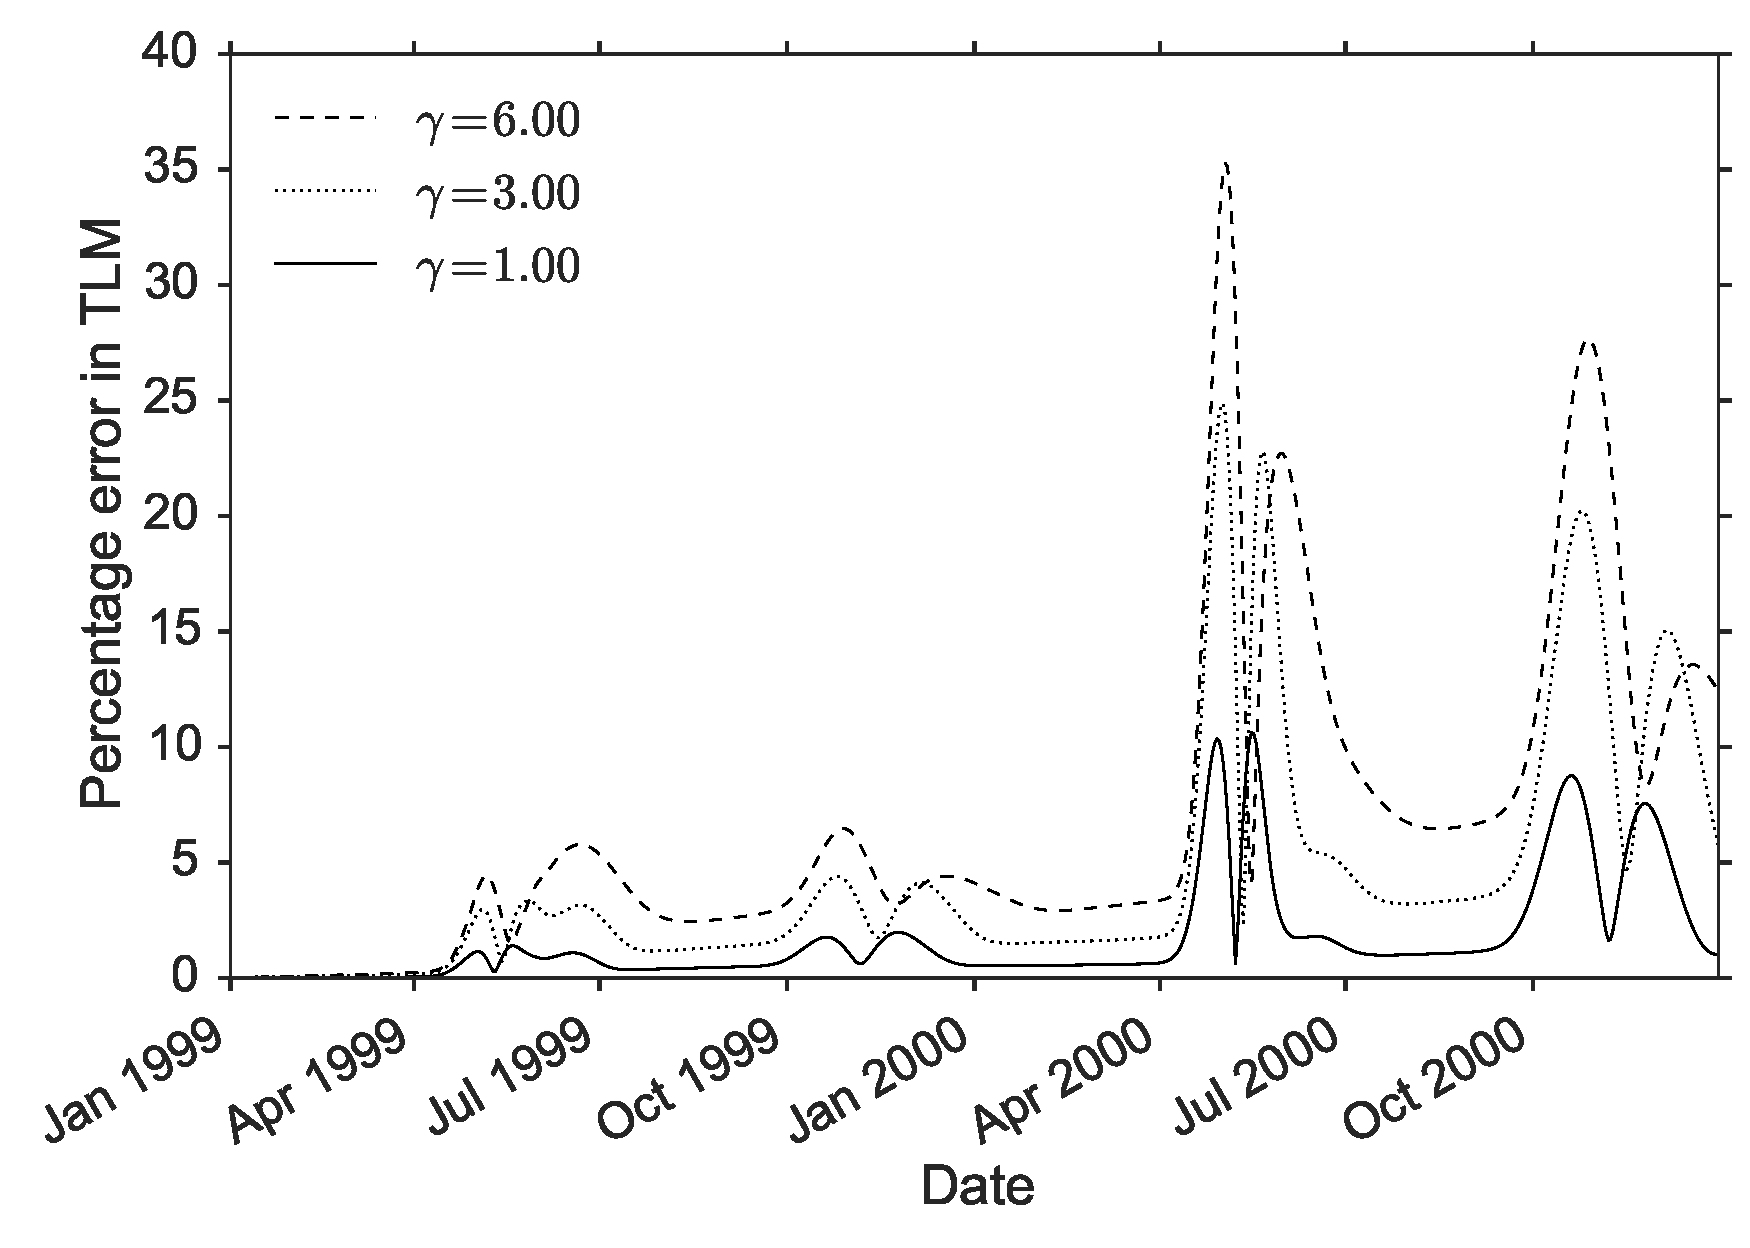
\includegraphics[width=0.5\textwidth]{percenterrlinmod.eps}
    \caption{Plot of the percentage error in the tangent linear model (equation \eqref{pertlmtest}) for DALEC2 when evolving the model state forward over a period of two years with three different values of $\gamma$ and a fixed $5\%$ perturbation $\delta \textbf{x}_0$.}
    \label{fig:tlm_error}
\end{figure}

In figure \ref{fig:tlm_error} we can see that the TLM for DALEC2 performs well after being run forward a year with less than a $7\%$ error for all values of $\gamma$. By the second year we see some peaks in the error in spring and autumn. This is due to leaf on and leaf off functions in the TLM going out of phase with the nonlinear DALEC2. At these peaks the error reaches a maximum at $35\%$ then coming back to around $10\%$ before growing again in the autumn. {\color{red} Although this level of error is still acceptable we present results using a one year assimilation window in this paper as in practice we could cycle assimilation windows to make use of multiple years of data \citep{moodycycled4dvar}. *rev3} 

\subsubsection{Test of adjoint model} 

The adjoint model we have implemented for DALEC2 passes correctness tests. For the TLM $\mathbf{M}_{i,0}$ and its adjoint $\mathbf{M}_{i,0}^{T}$ we have the identity
\begin{linenomath}
\begin{equation}
<\mathbf{M}_{i,0}\delta\textbf{x}_0, \mathbf{M}_{i,0}\delta\textbf{x}_0> = <\delta\textbf{x}_0, \mathbf{M}_{i,0}^{T}\mathbf{M}_{i,0}\delta\textbf{x}_0> \label{eqn:adjoint_test}
\end{equation}
\end{linenomath}
for any inner product $<, >$ and perturbation $\delta \textbf{x}_0$. This is derived from the adjoint identity \citep{lawless2013}. Using the Euclidean inner product, equation~\eqref{eqn:adjoint_test} is equivalent to
\begin{linenomath}
\begin{equation}
(\mathbf{M}_{i,0}\delta\textbf{x}_0)^{T} (\mathbf{M}_{i,0}\delta\textbf{x}_0) = \delta\textbf{x}_0^{T} (\mathbf{M}_{i,0}^{T}(\mathbf{M}_{i,0}\delta\textbf{x}_0)).
\end{equation}
\end{linenomath}
We evaluated the left hand side and right hand side of this identity for differing values of $\textbf{x}_0$ and size of perturbation $\delta \textbf{x}_0$ and showed that they were equal to machine precision.

\subsubsection{Gradient test} \label{sec:testgrad}

The 4D-Var system we have developed passes tests for the gradient of the cost function \citep{Navon1992}. In the implementation of the cost function and its gradient we regularise the problem using a variable transform \citep{Freitag2010}. For the cost function $J$ and its gradient $\nabla J$ we can show that we have implemented $\nabla J$ correctly using the identity,
\begin{linenomath}
\begin{equation}
f(\alpha)=\frac{| J( \textbf{x}_0 + \alpha \textbf{b}) - J(\textbf{x}_0) |}{\alpha \textbf{b}^{T} \nabla J(\textbf{x}_0)} = 1 + O(\alpha),
\end{equation}
\end{linenomath}
where $\textbf{b}$ is a vector of unit length and $\alpha$ is a parameter controlling the size of the perturbation. For small values of $\alpha$ not too close to machine precision we should have $f(\alpha)$ close to 1. Figure~\ref{fig:costone} shows $f(\alpha)$ for a 365 day assimilation window with $\textbf{b}=\textbf{x}_0||\textbf{x}_0||^{-1}$, we can see that $f(\alpha) \rightarrow 1$ as $\alpha \rightarrow 0$, as expected until $f(\alpha)$ gets too close to machine zero at order $\alpha = 10^{-11}$. This was also tested with $\textbf{b}$ in different directions and similar results obtained.

We can also plot $|f(\alpha)-1|$, where we expect $|f(\alpha)-1| \rightarrow 0$ as $\alpha \rightarrow 0$.  In figure~\ref{fig:cost} we have plotted $|f(\alpha)-1|$ for the same conditions as in figure~\ref{fig:costone}, we can see that $|f(\alpha) - 1| \rightarrow 0$ as $\alpha \rightarrow 0$, as expected (before $|f(\alpha)-1|$ gets too close to machine precision at order $\alpha = 10^{-8}$). This gives us confidence that the gradient of the cost function is implemented correctly.
%$\nabla J(\textbf{x}_0)||\nabla J(\textbf{x}_0)||^{-1}$. 

\begin{figure}[ht]
    \centering
    \begin{subfigure}[b]{0.49\textwidth}
        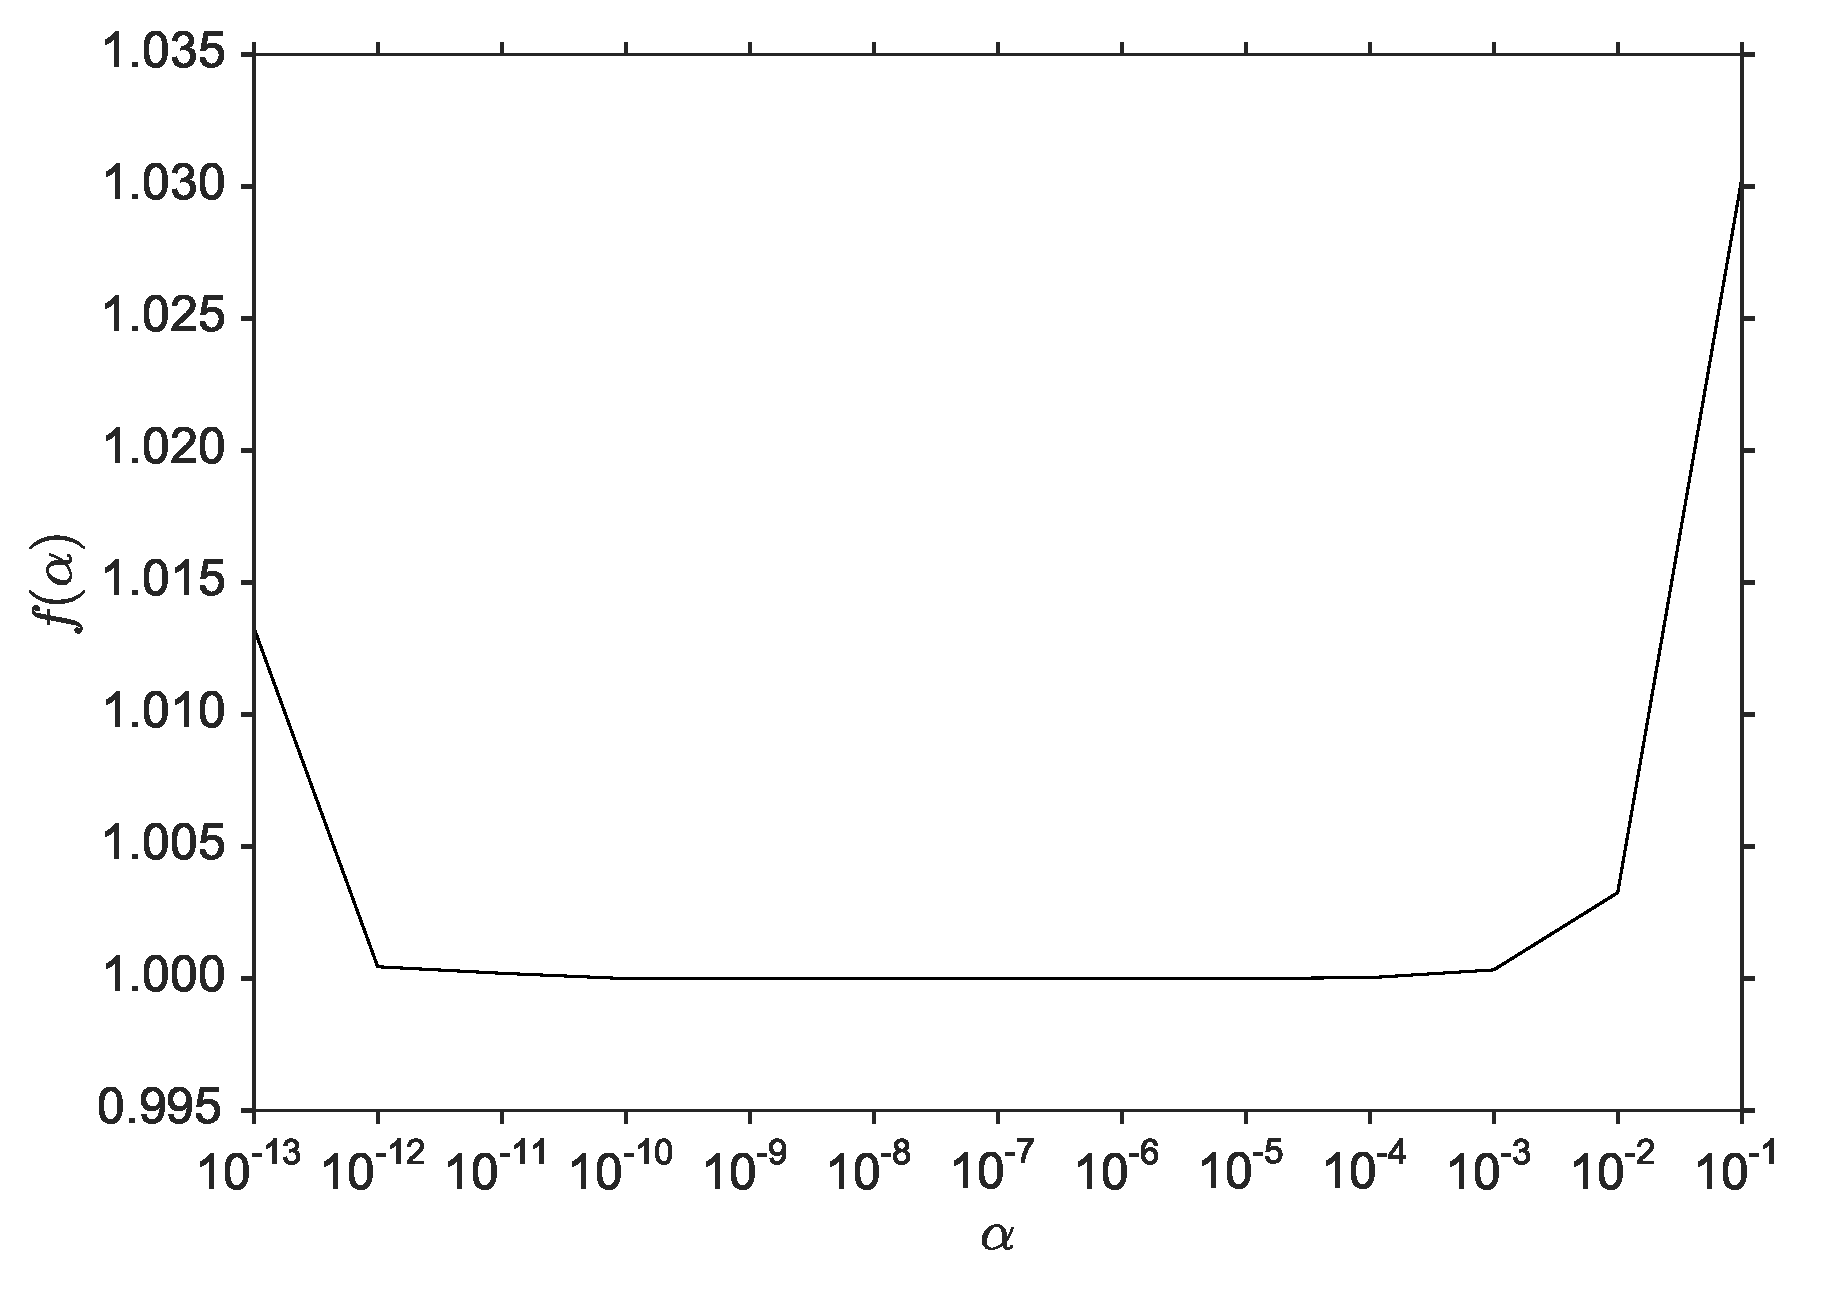
\includegraphics[width=\textwidth]{costone_cvt.eps}
        \caption{$f(\alpha)$ test}
        \label{fig:costone}
    \end{subfigure}
    \begin{subfigure}[b]{0.49\textwidth}
        \includegraphics[width=\textwidth]{cost_cvt.eps}
        \caption{$|f(\alpha) - 1|$ test}
        \label{fig:cost}
    \end{subfigure}
    \caption{Tests of the gradient of the cost function for a 365 day assimilation window with $\textbf{b}=\textbf{x}_0||\textbf{x}_0||^{-1}$.}
    \label{fig:testgradcostone}
\end{figure}

\subsection{Including correlations in the background error covariance matrix} \label{sec:corB}

As discussed in section~\ref{sec:intro}, including correlations in \textbf{B} impacts how information from assimilated observations is spread between different types of analysis variables \citep{bannister2008review}. We explored a number of different methods in order to include parameter-state correlations in \textbf{B}. In this paper we present a method using a set of ecological dynamical constraints, based on expert judgement, on model parameters and state variables from \citet{Bloom2015}. \citet{Bloom2015} show that implementing these constraints in a Metropolis Hastings MCMC data assimilation routine improves results significantly. The constraints impose conditions on carbon pool turnover and allocation ratios, steady state proximity and growth and the decay of model carbon pools.

In order to create a correlated background error covariance matrix, $\textbf{B}_{corr}$, using these constraints we create an ensemble of state vectors which we then take the covariance of to give us $\textbf{B}_{corr}$. To create this ensemble we use the following procedure:
\begin{enumerate}
\item Draw a random augmented state vector, $\textbf{x}_i$, from the multivariate truncated normal distribution described by
\begin{linenomath}
\begin{equation}
\textbf{x}_i \sim \mathcal{N}(\textbf{x}^b, \textbf{B}_{diag}),
\end{equation} 
\end{linenomath}
where $\textbf{B}_{diag}$ is the diagonal matrix described in section~\ref{sec:implement4dvar} and $\textbf{X}$ is bound by the parameter and state ranges given in table~\ref{table:xbvars} in the appendix.
\item Test this $\textbf{x}_i$ with the ecological dynamical constraints (requiring us to run the DALEC2 model using this state).
\item If $\textbf{x}_i$ passes it is added to our ensemble, else it is discarded.
\end{enumerate}
Once we have a full ensemble we then take the covariance of the ensemble to find $\textbf{B}_{corr}$. We chose an ensemble size of 1500 as {\color{red} a qualitative assessment of using a larger ensemble showed little difference in correlations. *rev3} In figure \ref{fig:Bcorr} we have plotted the correlation matrix or normalised error covariance matrix associated with $\textbf{B}_{corr}$. This matrix includes both positive and negative correlations between parameter and state variables, with correlations of 1 down the diagonal between variables of the same quantity as expected. The largest positive off-diagonal correlation is $0.42$ between $f_{lab}$ and $C_{lab}$. This makes physical sense as $f_{lab}$ is the parameter controlling the amount of GPP allocated to the labile carbon pool, $C_{lab}$.

\begin{figure}[ht]
    \centering
    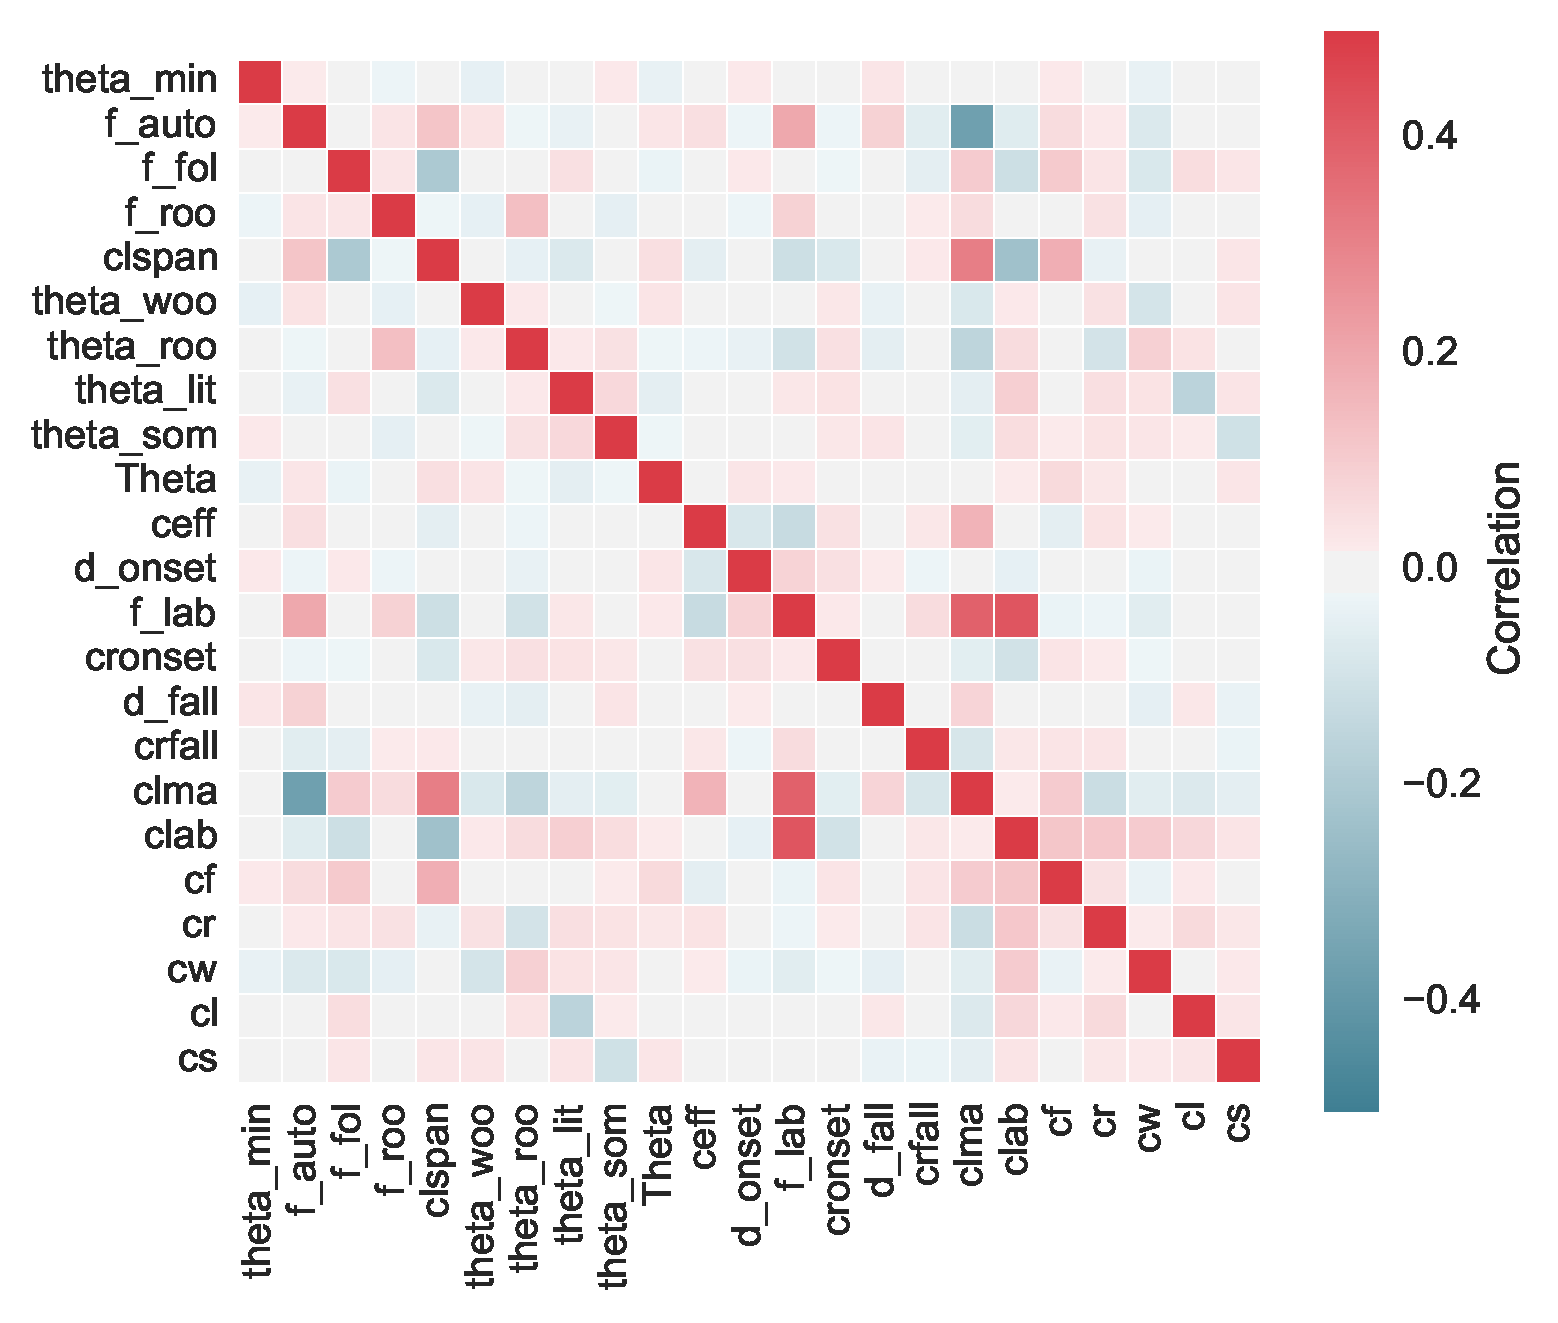
\includegraphics[width=0.55\textwidth]{bedccor.eps}
    \caption{Background error correlation matrix created using method in section \ref{sec:corB}. Here the correlation scale for off-diagonal values ranges from $-0.5$ to $0.5$ with the correlation along the diagonal being $1$. For explanation of parameter and state variable symbols see table~\ref{table:xbvars}.}
    \label{fig:Bcorr}
\end{figure}

\subsection{Specifying serial correlations in the observation error covariance matrix} \label{sec:corR}

The observation error covariance matrix does not only represent the instrumentation error for an observation but also the error in the observation operator (mapping the model state to the observation) and representativity error (error arising from the model being unable resolve the spatial and temporal scales of the observations). These other sources of error represented in $\hat{\textbf{R}}$ can also lead to correlations between observation errors \citep{Waller2014}. Errors in NEE observations come from different sources such as instrument errors, sampled ecosystem structure from the variable footprint of the flux tower and turbulent conditions (when there is low turbulence and limited air mixing the magnitude of NEE is underestimated). These errors due to turbulence can still have effect even after $u^{*}$ filtering \citep{Papale2006}. Due to this dependence on atmospheric conditions we expect the errors in observations of NEE to be serially correlated, as the atmospheric signal itself is serially correlated \citep{Daley1992}. If we were assimilating half hourly observations of NEE we would expect stronger correlations between observation errors, as atmospheric conditions are more constant at this time scale, with correlations between observation errors getting weaker with lower frequency observations. Although some studies suggest that the correlation between NEE measurement errors on the scale of a day is negligible \citep{lasslop:hal-00297973}, it is also likely that error in the observation operator and representativity error will lead to observation error correlations for NEE \citep{Waller2014}.

In section~\ref{4dvar} we have re-written the 4D-Var cost function in equation~\eqref{costfn} in order to allow the specification of serial observation error correlations in our assimilation scheme. These serial correlations are represented by the off-diagonal blocks of $\hat{\mathbf{R}}$. In work carried out with spatial correlations it has been shown that the structure of the correlation is not critical and that it is better to include some estimate of error correlation structure in the observation error covariance matrix than wrongly assume that errors are independent \citep{Stewart2013, Healy2005}. As a first attempt we try including temporal correlations on the scale of the observation frequency. We adapt the simple Gaussian model found in \citet{jarvinen1999variational} (a second order autoregressive correlation function was also tested but is not presented here). The correlation $r$ between 2 observations at times $t_1$ and $t_2$ is given as,
\begin{linenomath}
\begin{equation}
r =
\begin{cases} 
      a \text{exp} \bigg[ \frac{-(t_1 - t_2)^2}{\tau^2} \bigg] + (1- a)\delta_{t_1 - t_2} & |t_1 - t_2| \leq \eta \\
      0 & \eta < |t_1 - t_2| 
   \end{cases}
   , \label{eqn:corr_fn}
\end{equation}
\end{linenomath}
where $\tau$ is the e-folding time in days, $a$ controls the strength of correlation, $\delta$ is the Kronecker delta and $\eta$ is the cut off time after which the correlation between two observation errors is zero. We have incorporated a cut off for correlations between observation errors as the assumed correlation length scale for the assimilated observations is short. This cut off along with the form of correlation function using the Kronecker delta helps ensure $\hat{\mathbf{R}}$ is positive definite and therefore invertible, as required in the assimilation process. The standard deviation assumed in the observations of NEE is $0.5~\text{gCm}^{-2}\text{day}^{-1}$ as described in section~\ref{sec:implement4dvar}.

\begin{figure}[ht]
    \centering
    \includegraphics[width=0.5\textwidth]{rcorcor.eps}
    \caption{Observation error correlation matrix for the 67 observations used in assimilation created using method in section \ref{sec:corR} with $\tau = 4$, $a=0.3$ and $\eta=4$.}
    \label{fig:Rcorr}
\end{figure}

Figure~\ref{fig:Rcorr} shows the correlation matrix for $\hat{\mathbf{R}}$ created using equation~\eqref{eqn:corr_fn}. {\color{red} Here observations made on adjacent days will have an error correlation of 0.3, this will then decay exponentially for observations further apart in time. *rev3} There are 67 NEE observations in this one year assimilation window, these observations are not all on adjacent days and this is evident in the structure of $\hat{\mathbf{R}}$. The effect of the short e-folding time chosen here ($\tau=4$) provides the desired structure. 

\section{Results} \label{sec:results}

\subsection{Experiments} \label{sec:exps}

In the following sections we present the results of four experiments where we vary the representations of $\textbf{B}$ and $\hat{\mathbf{R}}$ while assimilating the same NEE observations in the window from the beginning of January 1999 to the end of December 1999. As shown in figure~\ref{fig:tlm_error} the performance of the tangent linear model deteriorates after the first year. We then forecast the NEE over the next 14 years (Jan 2000 - Dec 2013) and compare with the observed data. Using this shorter analysis window with a long forecast allows us to see the effect of including correlations in the error statistics more clearly, {\color{red} as we have a longer time-series of data with which to judge our forecast after data assimilation. *rev3} These experiments are outlined in table~\ref{table:exps_tab} where $\textbf{B}_{diag}$ and $\hat{\mathbf{R}}_{diag}$ are the diagonal matrices of the parameter and state variances and the observations variances respectively and $\textbf{B}_{corr}$ and $\hat{\mathbf{R}}_{corr}$ are the matrices as specified in section~\ref{sec:corB} and section~\ref{sec:corR} respectively.

\begin{table}[ht] 
\begin{center}
	\begin{tabular}{| l | l | l | l | l |}
	\hline
	Experiment & $\textbf{B}_{diag}$ & $\hat{\mathbf{R}}_{diag}$ & $\textbf{B}_{corr}$ &
	$\hat{\mathbf{R}}_{corr}$ \\ \hline
	A & $\times$ & $\times$ & & \\ \hline
	B & & $\times$ & $\times$ & \\ \hline
	C & $\times$ & & & $\times$ \\ \hline
	D & & & $\times$ & $\times$ \\ 
	\hline
	\end{tabular}
	\caption{The combination of error covariance matrices used in each data assimilation experiment.}
	\label{table:exps_tab}
\end{center} 
\end{table}

\subsection{Experiment A} \label{sec:expa}
In this experiment $\textbf{B}_{diag}$ and $\hat{\textbf{R}}_{diag}$ were used in the assimilation as described in section~\ref{sec:exps}. Because these contain no correlations this experiment forms the baseline by which the subsequent results from assimilation experiments are judged.  

Figure~\ref{fig:4dvardiagBR} shows assimilation and forecast results for NEE. We can see that assimilating the observations of NEE has improved the background with the analysis trajectory (green line) fitting well with the observations during the assimilation window (Jan 1999- Dec 1999). The analysis trajectory then diverges in the forecast (Jan 2000 - Dec 2013). This can be seen more clearly in figue~\ref{fig:broke4dvardiagBR}, where there is an over prediction of respiration in the winter and the seasonal cycle does not match that of the observations. {\color{red} This is also shown in figure~\ref{fig:Amoddat_resid} where we have plotted the model-data differences for a year's period averaged over the 14 years in the forecast period. Figure~\ref{fig:Amoddat_resid} shows that the largest errors in our posterior model forecast occur as a result of not capturing the phenology of the site correctly, in particular the start of the season from April to June. *rev3}
 
To see how well the forecast performs after assimilation we show a scatter plot of modelled NEE against observed NEE in figure~\ref{fig:forecastscatBR}. From table~\ref{table:results} the predictions have a Root-Mean-Square Error (RMSE) of $4.22 ~\text{gCm}^{-2}\text{day}^{-1}$ and a bias of $-0.3 ~\text{gCm}^{-2}\text{day}^{-1}$ for the forecast of NEE, whereas the analysis (Jan 1999 - Dec 1999) has a RMSE of $1.36 ~\text{gCm}^{-2}\text{day}^{-1}$ and a bias of $-0.03 ~\text{gCm}^{-2}\text{day}^{-1}$. The background or prior model trajectory meanwhile has a RMSE of $3.86 ~\text{gCm}^{-2}\text{day}^{-1}$ and a bias of $-1.60 ~\text{gCm}^{-2}\text{day}^{-1}$ in the analysis window (Jan 1999 - Dec 1999) and the same RMSE of $3.86 ~\text{gCm}^{-2}\text{day}^{-1}$ but a bias of $-1.36 ~\text{gCm}^{-2}\text{day}^{-1}$ during the forecast period (Jan 2000 - Dec 2013). Although using $\textbf{B}_{diag}$ and $\hat{\textbf{R}}_{diag}$ in the assimilation has considerably reduced the RMSE in the analysis period, it has also increased the RMSE in the forecast of NEE. However it has reduced the bias in the model forecast considerably from $-1.36 ~\text{gCm}^{-2}\text{day}^{-1}$ to $-0.3 ~\text{gCm}^{-2}\text{day}^{-1}$. The bias in the background is due to the background model predicting less negative values of NEE than observed (i.e. above the 1:1 line shown in figure~\ref{fig:forecastscatxb}). This leads to considerably worse results for the background trajectory than the analysis and its forecast for total forest carbon uptake. {\color{red} It is important to compare our results here with the background trajectory. The background trajectory acts as our initial prior model guess and is the starting point for our minimisation in 4D-Var. Comparing our assimilation results with our background trajectory give us confidence that our 4D-Var scheme is improving the results of our model after assimilation. *rev3}

\subsection{Experiment B} \label{sec:expb}

Here $\textbf{B}_{corr}$ (as defined in section~\ref{sec:corB}) and $\hat{\textbf{R}}_{diag}$ are used in the assimilation. Figure~\ref{fig:4dvaredcBR} shows assimilation and forecast results for NEE. In figure~\ref{fig:broke4dvaredcBR} we can see that the forecast performs considerably better than in experiment A, with the analysis trajectory no longer over predicting winter respiration and matching the observed seasonal cycle of NEE more closely in the forecast period (Jan 2000 - Dec 2013). {\color{red} This can be seen more clearly in figure~\ref{fig:Bmoddat_resid} where the improvement in the period April-June is considerable as we capture green-up at the site more closely. Even though we have improved the representation of leaf-on in our model significantly here we can see from figure~\ref{fig:broke4dvaredcBR} that this is still where we have the largest uncertainty for our model after assimilation. *rev3} From figure~\ref{fig:forecastscatedcBR} and table~\ref{table:results} we see that the forecast RMSE has almost halved (now $2.56 ~\text{gCm}^{-2}\text{day}^{-1}$) with a reduction in bias also, now $-0.2 ~\text{gCm}^{-2}\text{day}^{-1}$. In comparison using $\textbf{B}_{corr}$ in the assimilation very slightly degrades the fit for the analysis (Jan 1999 - Dec 1999), with a RMSE of $1.42 ~\text{gCm}^{-2}\text{day}^{-1}$ and a bias of $-0.04 ~\text{gCm}^{-2}\text{day}^{-1}$, as shown in table~\ref{table:results}. 

As discussed in section~\ref{sec:intro} previous work has shown the importance of specifying parameter-state correlations when using variational data assimilation for joint parameter and state estimation \citep{smith2009variational}. Although in 4D-Var some correlation structure may be added implicitly as $\textbf{B}_{diag}$ is evolved through time in experiment A, observations near the beginning of the window (before significant correlations develop in $\textbf{B}_{diag}$) will not be spread in a multivariate way. The correlations developed by the implicit evolution of $\textbf{B}_{diag}$ will also not include important physical relationships between variables. Therefore by not specifying these correlations in experiment A we allow the parameter and state variables to attain unrealistic values in order to find the best fit to the observations in the analysis window (Jan 1999 - Dec 1999), leading to the divergence seen in the forecast (1999-2014) in experiment A. {\color{red} It is important to note that even for longer time windows the implicit correlation structure that can be added by the 4d-Var algorithm will still not be enough to improve results considerably. Preconditioning of the background error covariance matrix is necessary in order to find the same level of improvement as the results presented here. *rev3}
 
We can see the effect that including correlations in $\textbf{B}$ has on the analysis update in figure~\ref{fig:xa_inc}. For some variables including correlations in $\textbf{B}$ has had a large impact on the analysis update after assimilation. This is particularly clear for the $f_{lab}$ parameter. The largest positive off-diagonal correlation in $\textbf{B}_{corr}$ is between $C_{lab}$ and $f_{lab}$, with $f_{lab}$ also having a large positive correlation with $c_{lma}$ as shown in section~\ref{sec:corB}. The effect of these correlations has been to change the analysis increment for $f_{lab}$ from being slightly positive in experiment A to being strongly negative by following the analysis update of its correlated variables $C_{lab}$ and $c_{lma}$. From figure~\ref{fig:xa_inc} we can also see some of the possible reasons for the improved fit to the observations in experiment B. {\color{red}From figure~\ref{fig:Amoddat_resid} the largest errors in our model forecast of NEE in experiment A stem from a misrepresentation of the phenology of the site in the months April-June. *rev3} We see that the parameter controlling day of leaf on ($d_{onset}$) has been updated slightly differently in comparison to experiment A, with day of leaf on now being slightly later in the year (day 124 instead of 119), again this is due to the included correlations in $\textbf{B}$. Even this small change in $d_{onset}$ appears to reduce the errors at the start of the season for experiment B as seen from figure~\ref{fig:Bmoddat_resid}. The forecast is also no longer over predicting winter respiration to the same extent as in experiment A. From figure~\ref{fig:xa_inc} we see that the main parameters controlling ecosystem respiration in NEE ($f_{auto}$, $\theta_{lit}$, $\theta_{som}$, $\Theta$) have been reduced in comparison with experiment A, which we believe have lead to an improved fit to observations in experiment B. In experiment A we also had an over prediction of peak carbon uptake in summer which has been improved in this experiment. From figure~\ref{fig:xa_inc} we see that one of the parameters controlling the magnitude of gross primary productivity ($c_{eff}$) has been decreased in comparison to experiment A. This appears to lead to less extreme predictions of peak summer carbon uptake than in experiment A.{\color{red} Two parameters with a significant change from experiment A are $f_{fol}$ and $C_{lit}$, however in \citet{Ann2013} the DALEC model prediction of NEE is shown to be largely insensitive to variations in these parameters. *rev3}

{\color{red}The added constraint provided by the correlations in $\textbf{B}_{corr}$ acts to regularise the data assimilation problem and avoid overfitting to the assimilated data by limiting the parameter space of the problem \citep{smith2009variational}. These correlations have been diagnosed using the EDC's from \citet{Bloom2015}, as shown in section~\ref{sec:corB}, so help to limit unrealistic behaviour for a mature forest site. *rev3} Although this has led to a slightly degraded fit to the observations in the analysis window (Jan 1999 - Dec 1999) it has also significantly improved the fit to observations for the forecast (Jan 2000 - Dec 2013).

\subsection{Experiment C} \label{sec:expc}

Here we use $\textbf{B}_{diag}$ and $\hat{\textbf{R}}_{corr}$ (as defined in section~\ref{sec:corR}) in the assimilation. Results shown in figure~\ref{fig:4dvarBcorR}, \ref{fig:broke4dvarBcorR} and \ref{fig:Cmoddat_resid} appear similar to those in section~\ref{sec:expa} however there are some differences. From table~\ref{table:results} and figure~\ref{fig:forecastscatBcorR} we see a slight reduction in RMSE for the forecast (now $4.09 ~\text{gCm}^{-2}\text{day}^{-1}$) in comparison with experiment A. As in experiment B the fit to the observations in the analysis window (Jan 1999 - Dec 1999) is very slightly degraded as the added correlations in $\hat{\textbf{R}}_{corr}$ act to reduce the weight of the observations in the assimilation \citep{jarvinen1999variational}. The changes seen when using $\hat{\textbf{R}}_{corr}$ in the assimilation are less than when using $\textbf{B}_{corr}$ as the correlations specified in $\hat{\textbf{R}}_{corr}$ are on a short timescale and much weaker than those in $\textbf{B}_{corr}$. In figure~\ref{fig:xa_inc} we can see that the changes between experiment A and C in the analysis increment are much less than when using $\textbf{B}_{corr}$.  

We also expect that specifying time correlations in $\hat{\textbf{R}}$ will help when assimilating other less frequently sampled data streams along with NEE as the serial correlations reduce the weight given to the mean of the more frequently sampled observations (here NEE) and also reduce the information content of these more frequently sampled observations \citep{jarvinen1999variational, Daley1992}, meaning that less frequently sampled data streams can have more impact on the assimilation.

\subsection{Experiment D}

In the final experiment we use $\textbf{B}_{corr}$ and $\hat{\textbf{R}}_{corr}$ in the assimilation. Figure~\ref{fig:broke4dvaredcBcorR}, figure~\ref{fig:broke4dvaredcBR} and \ref{fig:Amoddat_resid} shows that using both correlated matrices gives similar results as experiment B when $\textbf{B}_{corr}$ is used with $\hat{\textbf{R}}_{diag}$. However using $\hat{\textbf{R}}_{corr}$ in addition to $\textbf{B}_{corr}$ provides similar improvements as in experiment C. From table~\ref{table:results} and figure~\ref{fig:forecastscatedcBcorR} we see the forecast RMSE is slightly reduced again still from results in experiment B to $2.38 ~\text{gCm}^{-2}\text{day}^{-1}$. Using both matrices appears to combine the beneficial effects described in both section~\ref{sec:expb} and section~\ref{sec:expc}. In figure~\ref{fig:xa_inc} we can see that the analysis increment is very similar to experiment B.

\begin{figure}
    \centering
    \begin{subfigure}[b]{0.49\textwidth}
        \includegraphics[width=\textwidth]{A4dvar2.pdf}
        \caption{Experiment A}
        \label{fig:4dvardiagBR}
    \end{subfigure}
    \begin{subfigure}[b]{0.49\textwidth}
        \includegraphics[width=\textwidth]{B4dvar2.pdf}
        \caption{Experiment B}
        \label{fig:4dvaredcBR}
    \end{subfigure}
    \begin{subfigure}[b]{0.49\textwidth}
        \includegraphics[width=\textwidth]{C4dvar2.pdf}
        \caption{Experiment C}
        \label{fig:4dvarBcorR}
    \end{subfigure}
    \begin{subfigure}[b]{0.49\textwidth}
        \includegraphics[width=\textwidth]{D4dvar2.pdf}
        \caption{Experiment D}
        \label{fig:4dvaredcBcorR}
    \end{subfigure}
    \caption{One year assimilation and fourteen year forecast of Alice Holt NEE with DALEC2, blue dotted line: background model trajectory, green line: analysis and forecast after assimilation, grey shading: Error in model after assimilation (+/- 3 standard deviations), red dots: observations from Alice Holt flux site with error bars.}\label{fig:4dvar}
\end{figure}

\begin{figure}
    \centering
    \begin{subfigure}[b]{0.49\textwidth}
        \includegraphics[width=\textwidth]{Abroke4dvar2.pdf}
        \caption{Experiment A}
        \label{fig:broke4dvardiagBR}
    \end{subfigure}
    \begin{subfigure}[b]{0.49\textwidth}
        \includegraphics[width=\textwidth]{Bbroke4dvar2.pdf}
        \caption{Experiment B}
        \label{fig:broke4dvaredcBR}
    \end{subfigure}
    \begin{subfigure}[b]{0.49\textwidth}
        \includegraphics[width=\textwidth]{Cbroke4dvar2.pdf}
        \caption{Experiment C}
        \label{fig:broke4dvarBcorR}
    \end{subfigure}
    \begin{subfigure}[b]{0.49\textwidth}
        \includegraphics[width=\textwidth]{Dbroke4dvar2.pdf}
        \caption{Experiment D}
        \label{fig:broke4dvaredcBcorR}
    \end{subfigure}
    \caption{As figure~\ref{fig:4dvar} but only showing the first and final two years results from the one year assimilation and fourteen year forecast of Alice Holt NEE with DALEC2, blue dotted line: background model trajectory, green line: analysis and forecast after assimilation, grey shading: Error in model after assimilation (+/- 3 standard deviations), red dots: observations from Alice Holt flux site with error bars.}\label{fig:broke4dvar}
\end{figure}

\begin{figure}
    \centering
    \begin{subfigure}[b]{0.49\textwidth}
        \includegraphics[width=\textwidth]{Amoddat_resid.pdf}
        \caption{Experiment A}
        \label{fig:Amoddat_resid}
    \end{subfigure}
    \begin{subfigure}[b]{0.49\textwidth}
        \includegraphics[width=\textwidth]{Bmoddat_resid.pdf}
        \caption{Experiment B}
        \label{fig:Bmoddat_resid}
    \end{subfigure}
    \begin{subfigure}[b]{0.49\textwidth}
        \includegraphics[width=\textwidth]{Cmoddat_resid.pdf}
        \caption{Experiment C}
        \label{fig:Cmoddat_resid}
    \end{subfigure}
    \begin{subfigure}[b]{0.49\textwidth}
        \includegraphics[width=\textwidth]{Dmoddat_resid.pdf}
        \caption{Experiment D}
        \label{fig:Dmoddat_resid}
    \end{subfigure}
    \caption{Net ecosystem exchange model-data differences for the four experiments. Here each point corresponds to the mean model-data difference for that day of the year over the 14 year model forecast (Jan 2000 - Dec 2013).}\label{fig:broke4dvar}
\end{figure}

\begin{figure}
    \centering
     \begin{subfigure}[b]{0.4\textwidth}
        \includegraphics[width=\textwidth]{xbfscat2.pdf}
        \caption{Background}
        \label{fig:forecastscatxb}
    \end{subfigure}
    \begin{subfigure}[b]{0.4\textwidth}
        \includegraphics[width=\textwidth]{Afscat2.pdf}
        \caption{Experiment A}
        \label{fig:forecastscatBR}
    \end{subfigure}
    \begin{subfigure}[b]{0.4\textwidth}
        \includegraphics[width=\textwidth]{Bfscat2.pdf}
        \caption{Experiment B}
        \label{fig:forecastscatedcBR}
    \end{subfigure}
    \begin{subfigure}[b]{0.4\textwidth}
        \includegraphics[width=\textwidth]{Cfscat2.pdf}
        \caption{Experiment C}
        \label{fig:forecastscatBcorR}
    \end{subfigure}
    \begin{subfigure}[b]{0.4\textwidth}
        \includegraphics[width=\textwidth]{Dfscat2.pdf}
        \caption{Experiment D}
        \label{fig:forecastscatedcBcorR}
    \end{subfigure}
    \caption{Forecast scatter plot of modelled daily NEE vs. observations for Jan 2000 - Dec 2013 (green dots). Blue line represents the 1-1 line.}\label{fig:animals}
\end{figure}

\begin{figure}[ht]
    \centering
    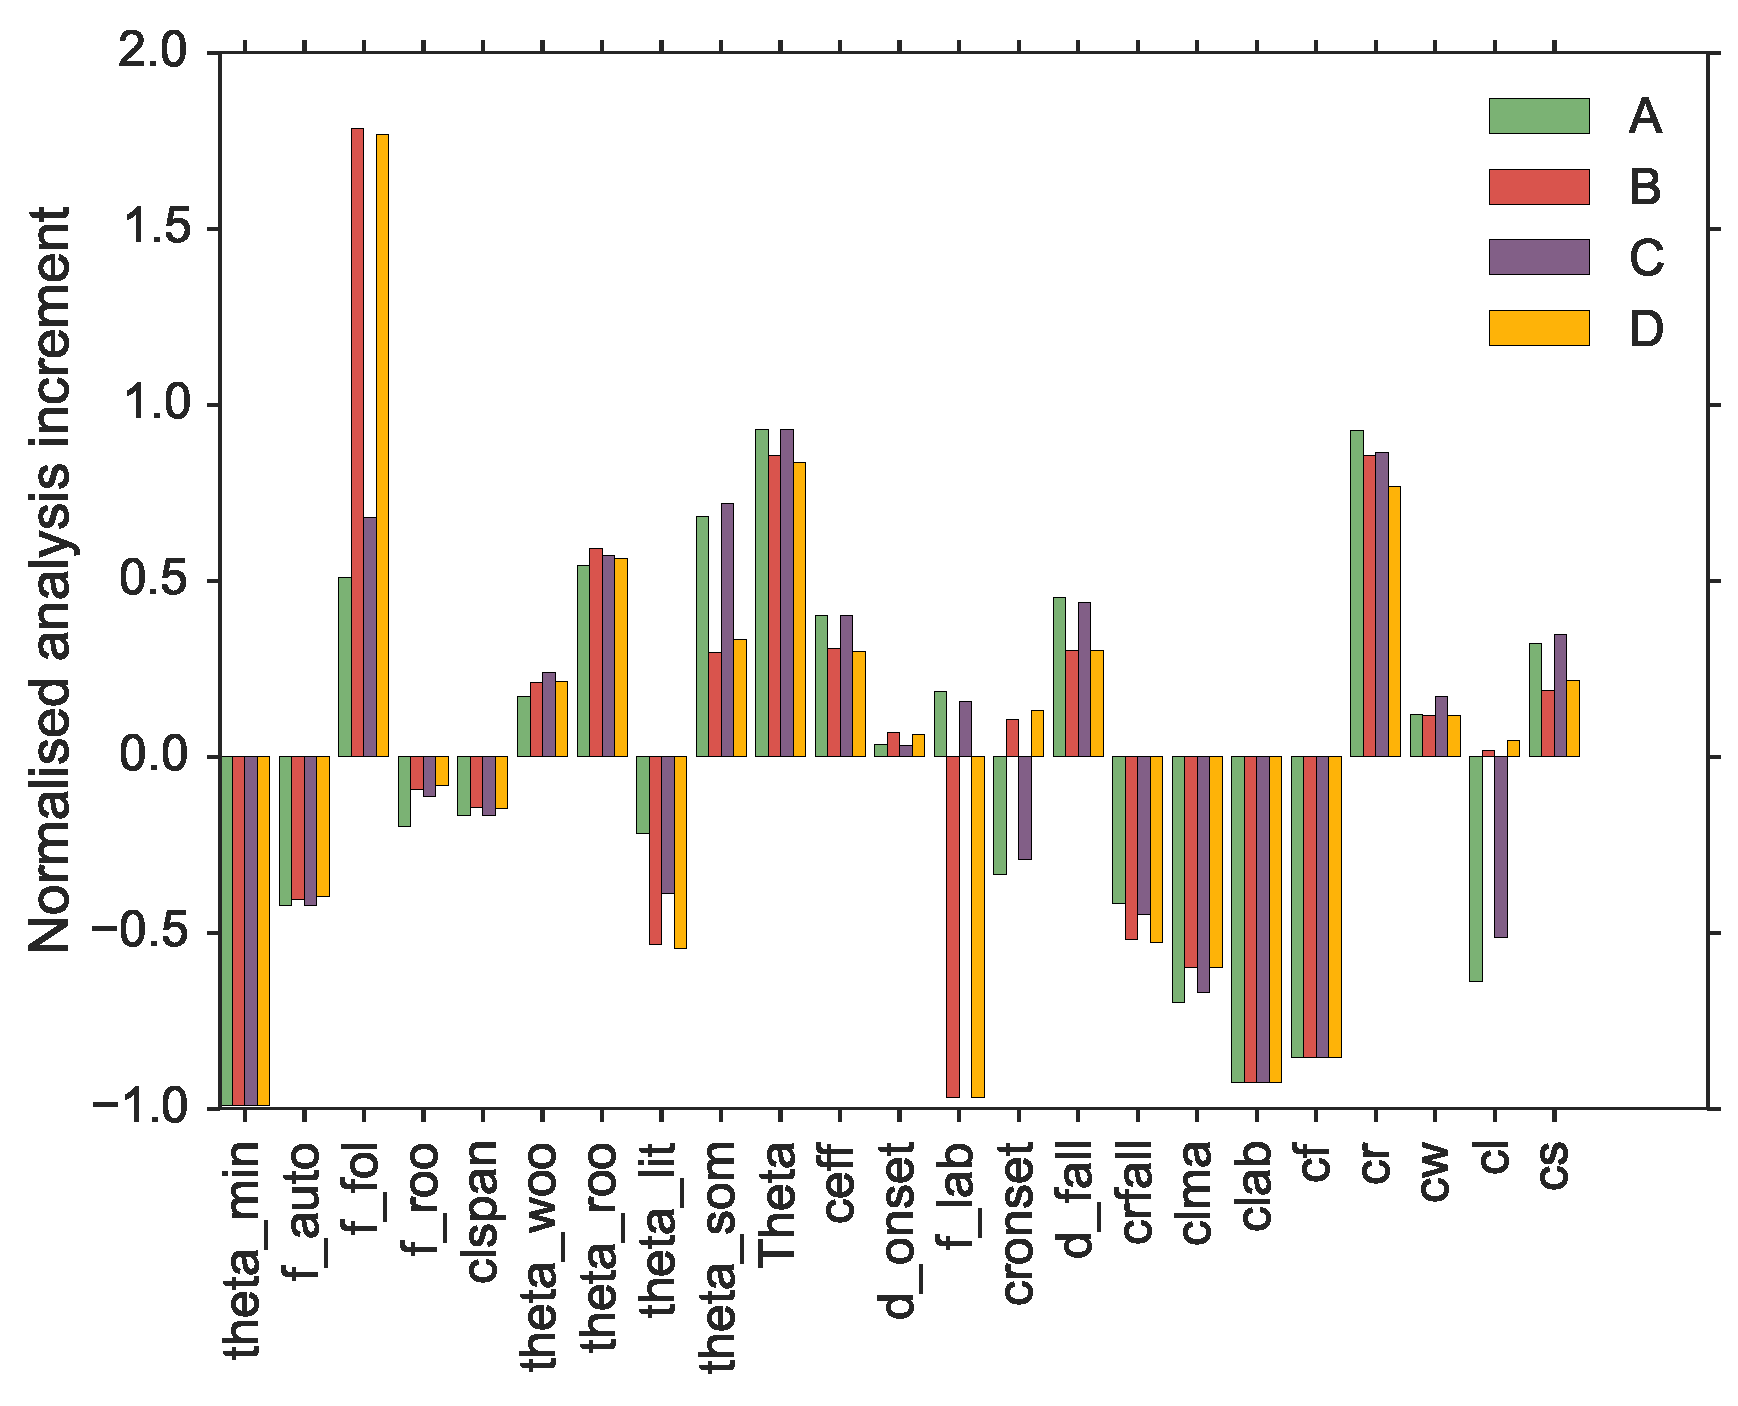
\includegraphics[width=0.8\textwidth]{inccvt.eps}
    \caption{Normalised analysis increment \big($\frac{(\textbf{x}^a - \textbf{x}^b)}{\textbf{x}^b}$\big) for the four experiments. Explanation of parameter and state variable symbols in table~\ref{table:xbvars}.}
    \label{fig:xa_inc}
\end{figure}

\subsection{Summary}

In our experiments we have shown that both $\textbf{B}_{corr}$ and $\hat{\textbf{R}}_{corr}$ have the effect of improving the model forecast of NEE. As it can be difficult to inspect the skill of a certain model by only plotting model trajectories, in figure~\ref{fig:taylordiag} we show Taylor diagrams displaying a statistical comparison of the four experiment and background analysis (Jan 1999 - Dec 1999) and forecast (Jan 2000 - Dec 2013) results with the observations of NEE. Here the radial distances from the origin to the points are proportional to the standard deviations of the observations and modelled observations and the azimuthal positions give the correlation coefficient between the modelled and observed NEE \citep{Taylor2001}. If a model predicted the observations perfectly it would have a correlation coefficient of $1$ and a radial distance matching that of the observations (represented by the dotted line). Figure~\ref{fig:td_a} shows that all the experiments give very similar results in the analysis window (Jan 1999 - Dec 1999) with all the experiment points closely grouped on top of each other, whereas figure~\ref{fig:td_f} shows the significant difference between the experiment results in the forecast (Jan 2000 - Dec 2013), with experiments B and D being closer to the dotted line. {\color{red} In all our experiments we find that $\theta_{min}$, $C_{lab}$ and $C_{fol}$ reach the bounds after assimilation. In the case of $\theta_{min}$ this is most likely due to the fact that we do not have enough information to recover this parameter when only assimilating observations of NEE, as the DALEC model prediction of NEE is insensitive to variations in this parameter \citep{Ann2013}. Assimilating more distinct data streams could help avoid this edge-hitting behaviour. For $C_{lab}$ and $C_{fol}$ this could suggest a flaw in the model or the fact that the prescribed bounds need to be relaxed slightly for the studied ecosystem. Our hypothesis is that the mechanism by which $C_{lab}$ is distributed to the leaves is over simplified, we intend to test this in future work. In table~\ref{table:expvars} we show the standard deviations for our parameter and state variables after assimilation. We can see that we have improved our confidence for most of these variables after assimilation when compared with the standard deviations in table~\ref{table:xbvars}. *rev3}

\begin{figure}[ht]
    \centering
    \begin{subfigure}[b]{0.49\textwidth}
        \includegraphics[width=\textwidth]{tdcvt_a.eps}
        \caption{Analysis (Jan 1999 - Dec 1999)}
        \label{fig:td_a}
    \end{subfigure}
    \begin{subfigure}[b]{0.49\textwidth}
        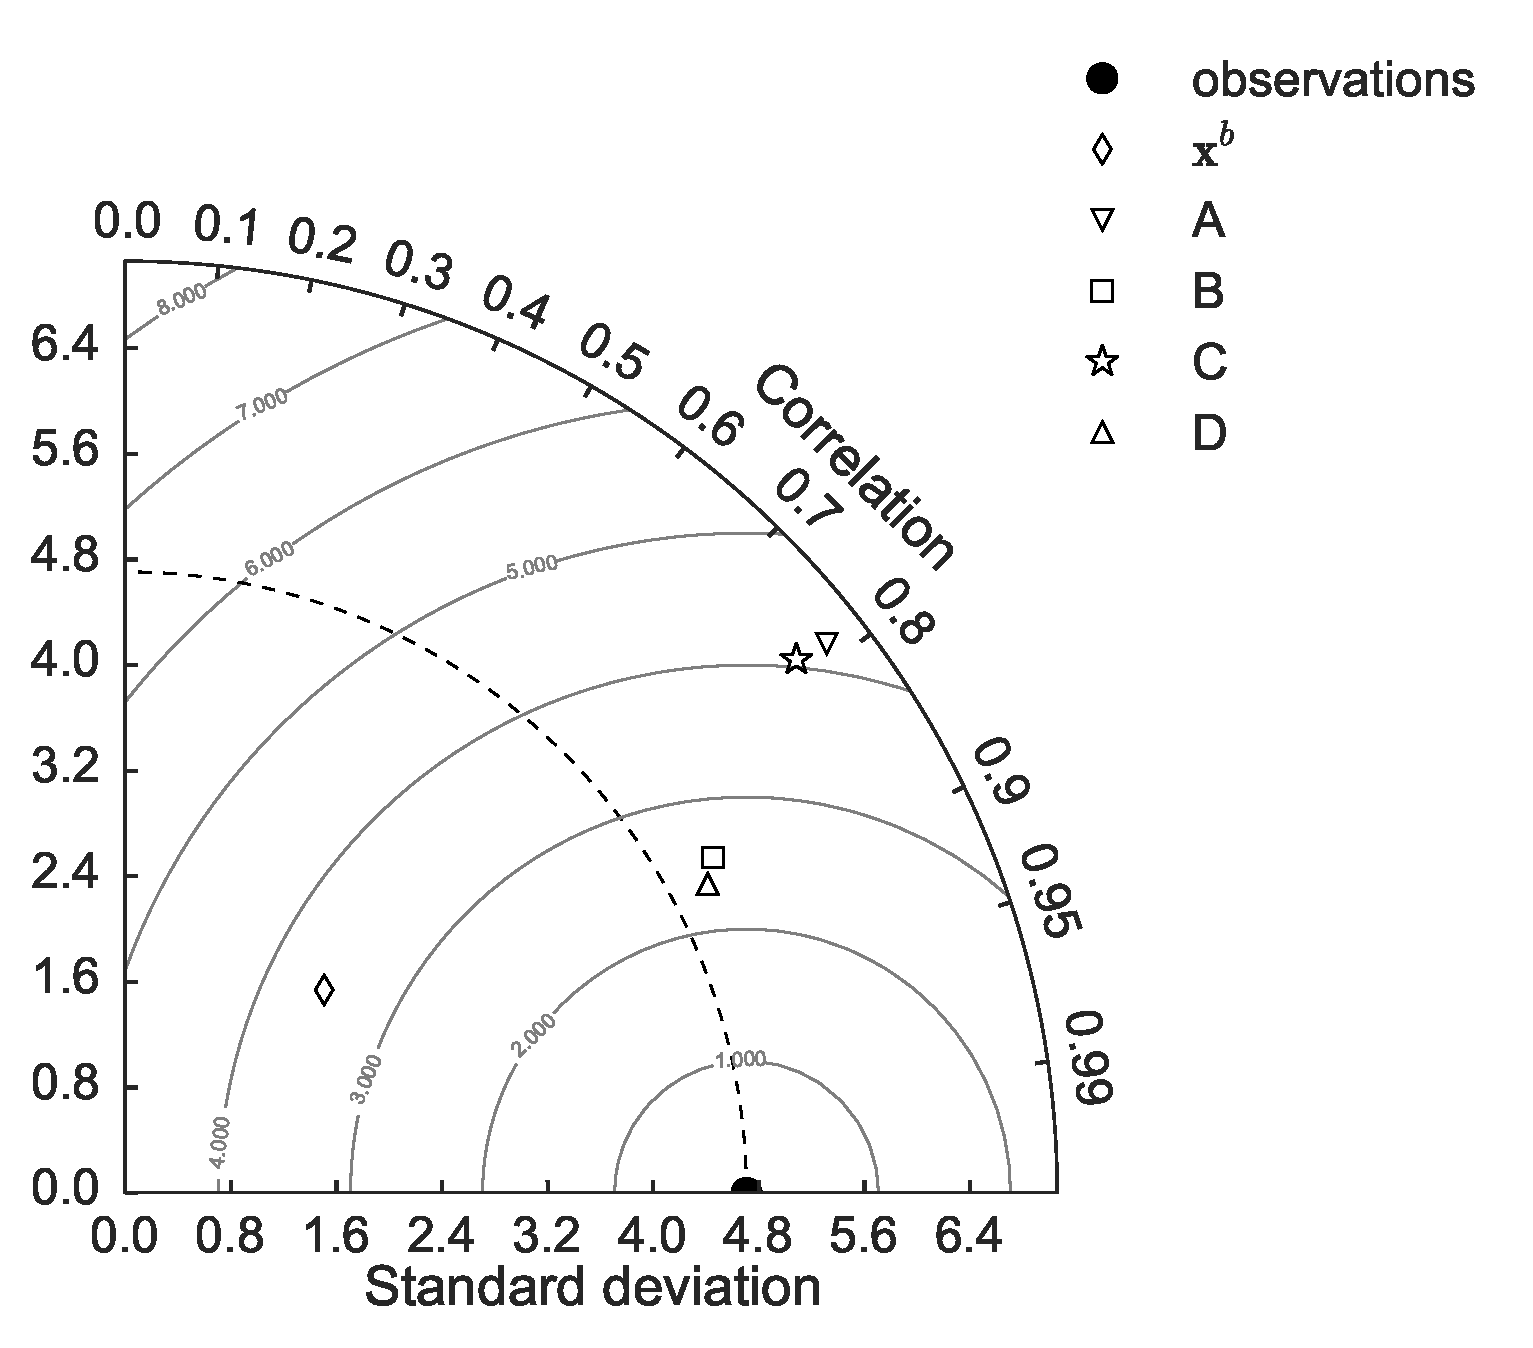
\includegraphics[width=\textwidth]{tdcvt_f.eps}
        \caption{Forecast (Jan 2000 - Dec 2013)}
        \label{fig:td_f}
    \end{subfigure}
    \caption{Taylor diagrams displaying statistical comparison of the four experiment and background analysis (Jan 1999 - Dec 1999) and forecast (Jan 2000 - Dec 2013) results with observations of NEE $( \text{gCm}^{-2}\text{day}^{-1})$. The dotted line represents the standard deviation of the observations and the contours represent values of constant root mean square error between model and observations.}
    \label{fig:taylordiag}
\end{figure}

\begin{table}[ht] 
\begin{center}
	\begin{tabular}{| l | l | l | l |}
	\hline
	\multicolumn{4}{| c |}{Analysis (Jan 1999 - Dec 1999)} \\ \hline
	Experiment & RMSE $( \text{gCm}^{-2}\text{day}^{-1})$ & Bias $( \text{gCm}^{-2}\text{day}^{-1})$ & Correlation coefficient \\ \hline
	Background & $3.86$ & $-1.60$ & $0.70$ \\ \hline
	A & $1.36$ & $-0.03$ & $0.96$ \\ \hline
	B & $1.42$ & $-0.04$ & $0.95$ \\ \hline
	C & $1.37$ & $-0.09$ & $0.96$ \\ \hline
	D & $1.43$ & $-0.09$ & $0.95$ \\ \hline
	\multicolumn{4}{| c |}{Forecast (Jan 2000 - Dec 2013)} \\ \hline
	Experiment & RMSE $( \text{gCm}^{-2}\text{day}^{-1})$ & Bias $( \text{gCm}^{-2}\text{day}^{-1})$ &  Correlation coefficient \\ \hline
	Background & $3.86$ & $-1.36$ & $0.66$ \\ \hline
	A & $4.22$ & $-0.30$ & $0.79$ \\ \hline
	B & $2.56$ & $-0.20$ & $0.87$ \\ \hline
	C & $4.09$ & $-0.51$ & $0.78$ \\ \hline
	D & $2.38$ & $-0.33$ & $0.88$ \\ 
	\hline
	\end{tabular}
	\caption{Analysis (Jan 1999 - Dec 1999) and forecast (Jan 2000 - Dec 2013) results for experiments and background when judged against observed NEE.}
	\label{table:results}
\end{center} 
\end{table}


\section{Discussion}

In this paper we have implemented the DALEC2 functional ecology model in a 4D-Var data assimilation scheme, building an adjoint of the DALEC2 model and applying rigorous tests to our scheme. Using 4D-Var can provide much faster assimilation results than MCMC techniques as we have knowledge of the derivative of the model. For our experiments the 4D-Var routine has taken in the order of $10^{2}$ function evaluations to converge to a minimum, whereas MCMC techniques using the same model take in the order of $10^{8}$ function evaluations \citep{Bloom2015}. However, we do assume that the statistics of the problem are Gaussian whereas MCMC techniques do not. We have shown that 4D-Var is a valid tool for improving the DALEC2 model estimate of NEE and that even when assimilating only a single year of NEE observations we can improve the forecast significantly. {\color{red} If more than one year was required this type of data assimilation routine could be run in cycling mode, allowing for the assimilation of multiple years of data. Cycling of 4D-Var involves running the analysis from the first year as the background for the second then iterating this until all desired data is assimilated \citep{moodycycled4dvar}, this also avoids any possible unstable behaviour associated with much longer single assimilation windows. *rev1} However, here our aim is to investigate the effect of specifying correlations in background and observation error statistics on the forecast of NEE. We have therefore assimilated just one year of NEE observations and produced a long 14 year forecast in order to see more clearly the effect of including these correlations on the forecast when judging against observations. The observations of daily NEE from the Alice Holt flux site are quite variable year to year, peak summer uptake varies from $-14.35~\text{gCm}^{-2}\text{day}^{-1}$ to $-9.04~\text{gCm}^{-2}\text{day}^{-1}$, and therefore provide a reasonable test for the ability of the DALEC2 model forecast, especially over a 14 year period.  

We then considered the nature of background and observation errors. The effect of specifying parameter-state correlations in the background information and serial correlations between the observation errors was explored.

The technique presented here to specify ${\mathbf{B}}_{corr}$ has been shown to have significantly improved forecasts of NEE over using a diagonal representation of ${\mathbf{B}}$. In section~\ref{sec:expb} we discuss how the correlations in ${\mathbf{B}}_{corr}$ impact the analysis update for the parameter and state variables (see figure~\ref{fig:xa_inc}) causing the seasonal cycle of carbon uptake and magnitude of fluxes to fit more closely with the observations than when using a diagonal ${\mathbf{B}}$ in the assimilation algorithm. These results agree with those of \citet{smith2009variational} where the importance of specifying parameter-state correlations when performing joint parameter and state estimation with variational data assimilation was shown. {\color{red} The added constraint provided by including correlations in $\textbf{B}$ acts to regularise the assimilation problem. This means the initial parameter and state values we retrieve from our data assimilation are more likely to be realistic, leading to better insight into the studied system. *rev1 }The method for specifying ${\mathbf{B}}_{corr}$ in this paper used a series of ecological dynamical constraints taken from \citet{Bloom2015}. {\color{red} Implementing correlations in the prior error statistics in this way may prove difficult for models where these type of constraints are not available, however there are other methods to build correlations into $\textbf{B}$. *rev1} One technique we also tested (not presented here) to create a correlated $\textbf{B}$ involved evolving an ensemble of state vectors over the length of the chosen assimilation window using the model (DALEC2) and then taking the covariance of the evolved ensemble. This gave us a \textbf{B} with parameter-state and state-state correlations, but no parameter-parameter correlations as the parameters are not updated by the model. Using the $\textbf{B}$ created with this method also improved assimilation results significantly over using a diagonal $\textbf{B}$. A larger number of different tests were run using different background vectors and variances and it was found that specifying some form of correlation structure in $\textbf{B}$ always made an improvement to the results of the assimilation. As this work has only considered a single deciduous site, it would be useful to apply the techniques detailed here for an evergreen site. Evergreen ecosystems usually have less extreme seasonal variation, it will therefore be of interest to see if a similar improvement for evergreen ecosystem forecast results is found when using a ${\mathbf{B}}_{corr}$ created using the same method.

The purpose of this exercise was to see how well we could forecast NEE while also investigating the effect of including correlations between error statistics. It was not an attempt to recover all the parameters and state variables with a high level of accuracy. However, it is still instructive to look at these values and compare with data where available. In \citet{meir2002acclimation} an observed range is given for leaf mass per area ($c_{lma}$) for the Alice Holt flux site of between $40$ to $80 ~\text{gCm}^{-2}$. The background value for $c_{lma}$ in our experiments is $128.5 ~\text{gCm}^{-2}$. When using diagonal error covariance matrices in experiment A we find a value of $38.7~\text{gCm}^{-2}$ for $c_{lma}$ after assimilation which is almost within the range given by \citet{meir2002acclimation}. In experiment D when using error covariance matrices including correlations $c_{lma}$ has a value of $51.6~\text{gCm}^{-2}$ after assimilation, this is well within the observed range given by \citet{meir2002acclimation}. From observations made by Forest Research we also have estimates to the above and below ground woody carbon pool ($C_{woo}$) at the start of 1999, with an observed value of $14258~\text{gCm}^{-2}$. It is not clear how uncertain this estimate is. The background value for $C_{woo}$ in our experiments is $6506~\text{gCm}^{-2}$. When using diagonal error covariance matrices in experiment A we find a value of $7291~\text{gCm}^{-2}$ for $C_{woo}$, an increase but still far away from the observed estimate. In experiment D when using error covariance matrices including correlations $C_{woo}$ has a value of $7262~\text{gCm}^{-2}$ a similar result as experiment A. Here the assimilation has not been able to recover a value of $C_{woo}$ similar to that of the observed estimate. {\color{red} This is not necessarily of concern as we are not able to quantify the error in this observation. *rev3} {\color{red}Also we are assimilating observations of daily NEE only, NEE is the difference between Gross Primary Productivity (GPP) and Total ecosystem respiration (RT), (NEE = RT - GPP), with neither GPP nor RT being direct functions of $C_{woo}$. Therefore it is unlikely that we will recover an accurate value of $C_{woo}$, as the assimilated observations are not significantly impacted by large changes in this state variable, this result is also discussed in \citet{fox2009reflex}. *rev3} This may also explains why we are able to recover a reasonable value of $c_{lma}$ from the assimilation, as from equation~\eqref{GPP} we can see that $c_{lma}$ is one of the input arguments taken by GPP. The function calculating NEE will therefore be sensitive to variations in the $c_{lma}$ parameter and so assimilating observations of NEE could help to constrain this parameter.

In numerical weather prediction it has been shown that including correlations in $\textbf{R}$ can help improve data assimilation results \citep{weston2014accounting, Stewart2013}. However the specified correlations have most commonly been satellite interchannel correlations with observations errors still being considered independent in time. In this paper we have shown that including correlations between observation errors in time can also improve data assimilation results, here providing a slight improvement for the DALEC2 model forecast of NEE. {\color{red} Here we only see a small impact on our results when using $\hat{\mathbf{R}}_{corr}$ in the assimilation as the correlations we have included are weak (especially in comparison to those included in ${\mathbf{B}}_{corr}$)  and on a short time-scale. We expect including correlations in $\hat{\textbf{R}}$ will have more of an impact on data assimilation results when assimilating data with stronger error correlations (i.e. finer temporal-resolution observations). We also expect including these serial correlations to have an even greater impact when assimilating more than one data stream as discussed in section~\ref{sec:intro}. *rev3} Using the form of $\hat{\mathbf{R}}$ given in this paper for specifying serial correlations will also allow us to specify serial correlations between different observation types. When running the DALEC2 model with a day-night time step, instead of the daily time step used for this paper, this will allow us to build in the type of correlations investigated by \citet{Baldocchi2015} between ecosystem respiration and canopy photosynthesis. More work is needed to investigate the effect of including correlations between observations error statistics when assimilating multiple data streams.

The $\hat{\mathbf{R}}_{corr}$ presented in this paper has a weak correlation ($a=0.3$ as shown in section\ref{sec:corR}) in time between observations of NEE, this representation of $\hat{\mathbf{R}}_{corr}$ has slightly improved the model forecast of NEE. However other choices of $\hat{\mathbf{R}}_{corr}$ (with much stronger correlations between observations) tested for this paper degraded the forecast. This is probably due to the specified correlations being unrealistic and highlights the fact that a reasonable estimate to the true correlation structure for $\hat{\mathbf{R}}_{corr}$ is needed to have a positive impact on results. The development of a more diagnostic approach for the calculation of serial correlations in $\hat{\mathbf{R}}$ would be useful. One option would be to adapt the \citet{desroziers2005diagnosis} diagnostic, which has been used successfully in numerical weather prediction for diagnosing observation error correlations for observations taken at the same time \citep{weston2014accounting}, and extending this technique to diagnose serial correlations. This will form the basis of future work. 

\section{Conclusion}

Functional ecology and land surface model data assimilation routines largely treat prior estimates of parameter and state uncertainties and observation error statistics as independent and uncorrelated. In this paper we have shown the importance of including estimates to such correlations, especially between background parameter and state error statistics when performing joint parameter and state estimation.

When performing joint parameter and state estimation including correlations in the background error covariance matrix significantly improves the forecast after assimilation, in comparison to using a diagonal representation of $\textbf{B}$. Specifying serial time correlations between observation errors in $\hat{\textbf{R}}$ also improves the forecast and we expect these correlations to have a greater impact when assimilating more than one data stream. More work is needed to investigate the effect of including these correlations when assimilating multiple data streams. The development of a more diagnostic tool for the calculation of the error correlation structure in $\hat{\textbf{R}}$ is also important.  

When including both parameter-state correlations in $\textbf{B}$ and time correlations between observation errors in $\hat{\textbf{R}}$ and assimilating only a single year of NEE observations we can forecast 14 years of NEE observations with a root-mean square error of $2.38~\text{gCm}^{-2}\text{day}^{-1}$ and a correlation coefficient of $0.88$. This is a significant $44\%$ reduction in error from the results when using a $\textbf{B}$ and $\hat{\textbf{R}}$ with no specified correlations of $4.22~\text{gCm}^{-2}\text{day}^{-1}$ and a correlation coefficient of $0.79$.

\section{Acknowledgements}

This work was funded by the UK Natural Environment Research Council (NE/K00705X/1) with a CASE award from the UK Forestry Commission. Work also partly funded by the National Centre for Earth Observation. We are grateful to Luke Smallman for providing the background information used in the experiments detailed in this paper.

\section*{References}

\bibliography{PhD}

\newpage

\section*{Appendix}

\begin{table}[ht] 
\begin{center}
	\begin{tabular}{| l | l | l | l | l |}
	\hline
	Parameter & Description & \pbox{7cm}{Background\\ vector ($\textbf{x}^{b}$)} & \pbox{7cm}{Standard \\deviation} & Range \\ \hline
$\theta_{min}$ & Litter mineralisation rate (day$^{-1}$) & $9.810\times 10^{-4}$ & $2.030\times 10^{-3}$ & $10^{-5} - 10^{-2}$ \\ \hline
$f_{auto}$ & Autotrophic respiration fraction & $5.190\times 10^{-1}$ & $1.168\times 10^{-1}$ & $0.3 - 0.7$  \\ \hline
$f_{fol}$ & Fraction of GPP allocated to foliage & $1.086\times 10^{-1}$ & $1.116\times 10^{-1}$ & $0.01-0.5$ \\ \hline
$f_{roo}$ & Fraction of GPP allocated to fine roots & $4.844\times 10^{-1}$ & $2.989\times 10^{-1}$ & $0.01-0.5$ \\ \hline
$c_{lspan}$ & Determines annual leaf loss fraction & $1.200\times 10^{0} $ & $1.161\times 10^{-1}$ & $1.0001 - 10$ \\ \hline
$\theta_{woo}$ & Woody carbon turnover rate (day$^{-1}$) & $1.013\times 10^{-4}$ & $1.365\times 10^{-4}$ & $2.5\times10^{-5} - 10^{-3}$ \\ \hline
$\theta_{roo}$ & Fine root carbon turnover rate (day$^{-1}$) & $3.225\times 10^{-3}$ & $2.930\times 10^{-3}$ & $10^{-4} - 10^{-2}$ \\ \hline
$\theta_{lit}$ & Litter carbon turnover rate (day$^{-1}$) & $3.442\times 10^{-3}$ & $3.117\times 10^{-3}$ & $10^{-4} - 10^{-2}$ \\ \hline
$\theta_{som}$ & Soil and organic carbon turnover rate (day$^{-1}$) & $1.113\times 10^{-4}$ & $1.181\times 10^{-4}$ & $10^{-7} - 10^{-3}$ \\ \hline
$\Theta$ & Temperature dependance exponent factor & $4.147\times 10^{-2}$ & $1.623\times 10^{-2}$ & $0.018 - 0.08$ \\ \hline
$c_{eff}$ & Canopy efficiency parameter & $7.144\times 10^{1}$ & $2.042\times 10^{1}$ & $10 - 100$ \\ \hline
$d_{onset}$ & Leaf onset day (day) & $1.158\times 10^{2}$ & $6.257\times 10^{0}$ & $1 - 365$ \\ \hline
$f_{lab}$ & Fraction of GPP allocated to labile carbon pool & $3.204\times 10^{-1}$ & $1.145\times 10^{-1}$ & $0.01 - 0.5$ \\ \hline
$c_{ronset}$ & Labile carbon release period (days) & $4.134\times 10^{1}$ & $1.405\times 10^{1}$ & $10 - 100$ \\ \hline
$d_{fall}$ & Leaf fall day (day) & $2.205\times 10^{2}$ & $3.724\times 10^{1}$ & $1 - 365$ \\ \hline
$c_{rfall}$ & Leaf-fall period (days) & $1.168\times 10^{2}$ & $2.259\times 10^{1}$ & $10 - 100$ \\ \hline
$c_{lma}$ & Leaf mass per area ($\text{gCm}^{-2}$) & $1.285\times 10^{2}$ & $6.410\times 10^{1}$ & $10 - 400$ \\ \hline
$C_{lab}$ & Labile carbon pool ($\text{gCm}^{-2}$) & $1.365\times 10^{2}$ & $6.626\times 10^{1}$ & $10 - 1000$ \\ \hline
$C_{fol}$ & Foliar carbon pool ($\text{gCm}^{-2}$) & $6.864\times 10^{1}$ & $3.590\times 10^{1}$ & $10 - 1000$ \\ \hline
$C_{roo}$ & Fine root carbon pool ($\text{gCm}^{-2}$) & $2.838\times 10^{2}$ & $2.193\times 10^{2}$ & $10 - 1000$ \\ \hline
$C_{woo}$ & Above and below ground woody carbon pool ($\text{gCm}^{-2}$) & $6.506\times 10^{3}$ & $7.143\times 10^{3}$ & $100 - 10^{5}$ \\ \hline
$C_{lit}$ & Litter carbon pool ($\text{gCm}^{-2}$) & $5.988\times 10^{2}$ & $5.450\times 10^{2}$ & $10 - 1000$ \\ \hline
$C_{som}$ & Soil and organic carbon pool ($\text{gCm}^{-2}$) & $1.936\times 10^{3}$ & $1.276\times 10^{3}$ & $100 - 2 \times 10^{5}$  \\ \hline
	\end{tabular}
	\caption{Parameter values and standard deviations for background vector used in experiments.}
	\label{table:xbvars}
\end{center} 
\end{table}

\begin{table}[ht] 
\begin{center}
	\begin{tabular}{| l | l | l | l | l |}
	\hline
	Parameter & A & B & C & D \\ \hline
$\theta_{min}$ & $1.822\times 10^{-6}$ & $3.742\times 10^{-7}$ & $1.519\times 10^{-6}$ & $3.854\times 10^{-7}$ \\ \hline
$f_{auto}$ & $2.913\times 10^{-3}$ & $1.428\times 10^{-3}$ & $2.937\times 10^{-3}$ & $1.510\times 10^{-3}$ \\ \hline
$f_{fol}$ & $5.459\times 10^{-3}$ & $4.581\times 10^{-3}$ & $6.797\times 10^{-3}$ & $4.591\times 10^{-3}$ \\ \hline
$f_{roo}$ & $7.907\times 10^{-2}$ & $9.141\times 10^{-3}$ & $8.199\times 10^{-2}$ & $9.149\times 10^{-3}$ \\ \hline
$c_{lspan}$ & $4.884\times 10^{-7}$ & $5.894\times 10^{-4}$ & $5.304\times 10^{-7}$ & $5.469\times 10^{-4}$ \\ \hline
$\theta_{woo}$ & $1.849\times 10^{-8}$ & $8.365\times 10^{-9}$ & $1.849\times 10^{-8}$ & $8.365\times 10^{-9}$ \\ \hline
$\theta_{roo}$ & $6.870\times 10^{-6}$ & $3.494\times 10^{-6}$ & $7.326\times 10^{-6}$ & $3.508\times 10^{-6}$ \\ \hline
$\theta_{lit}$ & $3.144\times 10^{-6}$ & $4.808\times 10^{-7}$ & $2.242\times 10^{-6}$ & $4.635\times 10^{-7}$ \\ \hline
$\theta_{som}$ & $1.178\times 10^{-8}$ & $6.848\times 10^{-9}$ & $1.210\times 10^{-8}$ & $6.850\times 10^{-9}$ \\ \hline
$\Theta$ & $7.905\times 10^{-5}$ & $6.808\times 10^{-5}$ & $8.010\times 10^{-5}$ & $6.978\times 10^{-5}$ \\ \hline
$c_{eff}$ & $3.755\times 10^{2}$ & $2.625\times 10^{2}$ & $3.724\times 10^{2}$ & $2.608\times 10^{2}$ \\ \hline
$d_{onset}$ & $3.552\times 10^{1}$ & $3.755\times 10^{1}$ & $3.649\times 10^{1}$ & $3.766\times 10^{1}$ \\ \hline
$f_{lab}$ & $1.220\times 10^{-2}$ & $3.209\times 10^{-3}$ & $1.225\times 10^{-2}$ & $3.203\times 10^{-3}$ \\ \hline
$c_{ronset}$ & $8.304\times 10^{1}$ & $1.642\times 10^{2}$ & $1.100\times 10^{2}$ & $1.644\times 10^{2}$ \\ \hline
$d_{fall}$ & $5.992\times 10^{2}$ & $5.294\times 10^{1}$ & $5.772\times 10^{2}$ & $6.145\times 10^{1}$ \\ \hline
$c_{rfall}$ & $1.540\times 10^{2}$ & $1.521\times 10^{2}$ & $1.604\times 10^{2}$ & $1.599\times 10^{2}$ \\ \hline
$c_{lma}$ & $2.134\times 10^{2}$ & $2.209\times 10^{2}$ & $2.503\times 10^{2}$ & $2.372\times 10^{2}$ \\ \hline
$C_{lab}$ & $6.142\times 10^{2}$ & $5.709\times 10^{2}$ & $8.586\times 10^{2}$ & $5.618\times 10^{2}$ \\ \hline
$C_{fol}$ & $7.971\times 10^{2}$ & $1.212\times 10^{2}$ & $8.029\times 10^{2}$ & $1.285\times 10^{2}$ \\ \hline
$C_{roo}$ & $3.984\times 10^{4}$ & $2.539\times 10^{4}$ & $4.114\times 10^{4}$ & $2.553\times 10^{4}$ \\ \hline
$C_{woo}$ & $5.075\times 10^{7}$ & $2.764\times 10^{7}$ & $5.075\times 10^{7}$ & $2.764\times 10^{7}$ \\ \hline
$C_{lit}$ & $4.157\times 10^{4}$ & $5.416\times 10^{4}$ & $7.179\times 10^{4}$ & $5.532\times 10^{4}$ \\ \hline
$C_{som}$ & $1.454\times 10^{6}$ & $1.106\times 10^{6}$ & $1.482\times 10^{6}$ & $1.105\times 10^{6}$  \\ \hline
	\end{tabular}
	\caption{Standard deviations for each experiment after assimilation, calculated using equation~\ref{eqn:Amat}.}
	\label{table:expvars}
\end{center} 
\end{table}



\end{document}